\documentclass[a4paper,12pt,onecolumn]{article}

\usepackage[T1]{fontenc}
\usepackage[utf8]{inputenc}
\usepackage[english]{babel}
\usepackage{amssymb,amsmath,amsthm,array,epsfig,lmodern,gensymb,pstricks,subfig,
hyperref,verbatim,booktabs,textcomp}

\newcommand{\R}{\mathbb R}
\newcommand{\D}{\mathcal D}
\newcommand{\W}{\vec{\mathcal W}}
\newcommand{\vol}{\mathcal{L}^d}
\newcommand{\surfvol}{\mathcal{H}^{d-1}}
\newcommand{\dH}[1]{\;{\rm d}{\cal H}^{#1}} % Hausdorff measure
\newcommand{\dL}[1]{\;{\rm d}{\cal L}^{#1}} % Lebesgue measure
\newcommand{\bigchi}{\ensuremath{\mathrm{\mathcal{X}}}}
\newcommand{\charfcn}[1]{\bigchi_{#1}} % characteristic function
\newcommand{\Vh}{\underline{V}(\Gamma^m)}
\newcommand{\Wh}{W(\Gamma^m)}
\newcommand{\Vht}{\underline{V}(\Gamma^h(t))}
\newcommand{\Wht}{W(\Gamma^h(t))}
\newcommand{\uspacesimple}{\mathbb{U}}
\newcommand{\uspace}[1]{\mathbb{U}(\vec{#1})}
\newcommand{\uspacedisc}[2]{\mathbb{U}^{#2}(\vec{#1})}
\newcommand{\pspace}{\mathbb{P}}
\newcommand{\pnormspace}{\widetilde\pspace} % normalized pressure space
\newcommand{\uspacesimpleref}{\mathcal{U}} % ale reference space
\newcommand{\uspaceref}[1]{\mathcal{U}(\vec{#1})} % ale reference space
\newcommand{\uspacesemidiscref}[2]{\mathcal{U}^{#2}(\vec{#1})}
% ale reference space
\newcommand{\pspaceref}{\mathcal{P}} % ale reference space
\newcommand{\pnormspaceref}{\widetilde\pspaceref}% ale reference space
\newcommand{\uspacesimpleale}{\mathfrak{U}} % ale space
\newcommand{\uspaceale}[1]{\mathfrak{U}(\vec{#1})} % ale space
\newcommand{\uspacesemidiscale}[3]{\mathfrak{U}^{#2}(\vec{#1},#3)} % ale space
\newcommand{\uspacediscale}[2]{\mathfrak{U}^{#2}(\vec{#1})} % ale space
\newcommand{\pspaceale}{\mathfrak{P}} % ale space
\newcommand{\pnormspaceale}{\widetilde\pspaceale}% ale normalized space
\newcommand{\kspace}{\mathbb{K}}
\newcommand{\xspace}{\mathbb{X}}
\newcommand{\sigmaO}{o}
\newcommand{\nabs}{\nabla_{\!s}}
\newcommand{\id}{\rm id}
\newcommand{\ddt}{\frac{\rm d}{{\rm d}t}}
\newcommand{\NbulkT}{\vec{N}_{\Gamma,\Omega}^T}
\newcommand{\Nbulk}{\vec{N}_{\Gamma,\Omega}}
\newcommand{\errorXx}{\|\Gamma^h - \Gamma\|_{L^\infty}}
\newcommand{\LerrorUu}[1]{\|\vec U - I^h_{#1}\,\vec u\|_{L^2}}
\newcommand{\HerrorUu}[1]{\|\vec U - I^h_{#1}\,\vec u\|_{L^2(H^1)}}
\newcommand{\LerrorPp}{\|P - p\|_{L^2}}
\newcommand{\unitn}{\vec{\rm n}}
\newcommand{\unitt}{\vec{\rm t}}
\newcommand{\mat}[1]{\underline{\underline{#1}}\rule{0pt}{0pt}}
\newcommand{\Rey}{\mbox{\textit{Re}}} % Reynolds number
\newcommand{\V}{\vec{\mathcal{V}}} % surface velocity
\newcommand{\pdg}{${\rm P1}^{{\rm dg}_\Gamma}$} % P1 DG across interface
\newcommand{\strikes}{\mbox{$s\!\!\!\!\:/$}}

\newtheorem{thm}{Theorem}
\newtheorem{lem}[thm]{Lemma}
\newtheorem{rem}[thm]{Remark}

\newenvironment{keywords}{{\upshape\bfseries Key words. }\ignorespaces}{}

\renewcommand{\theequation}{\arabic{section}.\arabic{equation}}

\textwidth 425pt

\title{Fitted Finite Element Discretization of\\ Two-Phase Navier--Stokes Flow}
\author{Marco Agnese and Robert N\"urnberg%
\thanks{email: \texttt{\{m.agnese13,robert.nurnberg\}@imperial.ac.uk}}\\
\small
Department of Mathematics, Imperial College, London, SW7 2AZ, U.K.}
\date{}

\begin{document}

\captionsetup[subfigure]{labelformat=empty} % remove label subplot

\maketitle

\begin{abstract}
TODO
\end{abstract}

\begin{keywords}
viscous incompressible two-phase flow, Navier--Stokes equations,
free boundary problem, surface tension, finite elements, front tracking
\end{keywords}

\section{Mathematical model}\label{sec:ns_model}
In this paper We now consider two-phase Navier--Stokes flow in a given domain
$\Omega\subset\R^d$, where $d=2$ or $d=3$. The domain $\Omega$ contains two
different immiscible, incompressible fluids (liquid-liquid or liquid-gas) which
for all $t\in[0,T]$ occupy time dependent regions $\Omega_+(t)$ and
$\Omega_-(t):=\Omega\setminus\overline{\Omega}_+(t)$ and which are separated by
an interface $(\Gamma(t))_{t\in[0,T]}$, $\Gamma(t)\subset\Omega$. We limit
ourselves to interfaces formed by closed hypersurfaces, see
Figure~\ref{fig:two_phase_sketch} for a pictorial representation in dimension
$d=2$.
\begin{figure}
\begin{center}
\unitlength15mm
\psset{unit=\unitlength,linewidth=1pt}
\begin{picture}(4,4)(0,0)
\psline(0,0)(4,0)(4,4)(0,4)(0,0)
\psellipse(2,2)(1,1)
\psline{->}(3,2)(3.5,2)
\put(3.25,1.75){$\vec\nu$}
\put(1.75,0.75){{$\Gamma(t)$}}
\put(1.75,2){{$\Omega_-(t)$}}
\put(0.5,3.25){{$\Omega_+(t)$}}
\end{picture}
\end{center}
\caption{The domain $\Omega$ in the case $d=2$.}
\label{fig:two_phase_sketch}
\end{figure}
For later use, we assume that $(\Gamma(t))_{t\in [0,T]}$ is a sufficiently
smooth evolving hypersurface without boundary that is parameterized by
$\vec x(\cdot,t):\Upsilon\to\R^d$, where $\Upsilon\subset \R^d$ is a given
reference manifold such that $\Gamma(t) = \vec x(\Upsilon,t)$. Then
\begin{equation} \label{eq:V}
\V(\vec z, t) := \vec x_t(\vec q, t) \quad
\forall\ \vec z = \vec x(\vec q,t) \in \Gamma(t)\,,
\end{equation}
defines the velocity of $\Gamma(t)$, and $\V \,.\,\vec \nu$ is
the normal velocity of the evolving hypersurface $\Gamma(t)$,
where $\vec\nu(t)$ is the unit normal on $\Gamma(t)$ pointing into
$\Omega_+(t)$.

Denoting the velocity and pressure by $\vec u$ and $p$, respectively, we
introduce the stress tensor
\begin{equation} \label{eq:stress_tensor}
\mat\sigma = \mu \,(\nabla\,\vec u + (\nabla\,\vec u)^T) - p\,\mat\id
= 2\,\mu\, \mat D(\vec u)-p\,\mat\id\,,
\end{equation}
where $\mu(t) = \mu_+\,\charfcn{\Omega_+(t)} + \mu_-\,\charfcn{\Omega_-(t)}$,
with $\mu_\pm \in \R_{>0}$, denotes the dynamic viscosities in the two phases,
$\mat\id \in \R^{d \times d}$ is the identity matrix and
$\mat D(\vec u):=\frac12\, (\nabla\vec u+(\nabla\vec u)^T)$
is the rate-of-deformation tensor.

The fluid dynamics in the bulk domain $\Omega$ are governed by the two-phase
Navier--Stokes model
\begin{subequations}
\begin{alignat}{2}
\rho\,(\vec u_t +(\vec u \,.\, \nabla)\vec u) -2 \mu\,\nabla\,.\,\mat D(\vec u)+
\nabla\,p & = \vec f \quad &&\mbox{in } \Omega_\pm(t)\,,
\label{eq:ns_momentum_bis} \\
\nabla\,.\,\vec u & = 0 \quad &&\mbox{in } \Omega_\pm(t)\,,
\label{eq:ns_mass_bis}
\end{alignat}
\end{subequations}
which describes the velocity $\vec u$ and pressure $p$ fields of the fluid. The
velocity and stress tensor need to be coupled across the free surface
$\Gamma(t)$. Viscosity of the fluids leads to the continuity condition
\begin{equation}\label{eq:interface_jump_velocity}
[\vec u]_-^+ = \vec 0 \quad \mbox{on } \Gamma(t)\,,
\end{equation}
where $[\vec u]_-^+ := \vec u_+ - \vec u_-$ denote the jump in velocity across
the interface $\Gamma(t)$. Here and throughout, we employ the shorthand notation
$\vec h_\pm := \vec h\!\mid_{\Omega_\pm(t)}$ for a function
$\vec h : \Omega \times [0,T] \to \R^d$; and similarly for scalar and
matrix-valued functions. The assumption that there is no change of phase leads
to the dynamic interface condition
\begin{equation}\label{eq:interface_velocity}
\V\,.\,\vec\nu = \vec u\,.\,\vec \nu \quad \mbox{on }
\Gamma(t)\,,
\end{equation}
which means that the normal velocity of the interface needs to match the flow
normal velocity across the interface $\Gamma(t)$. Moreover, the momentum
conservation in a small material volume that intersects the interface leads to
the stress balance condition
\begin{equation}\label{eq:interface_jump_stress_div}
[\mat\sigma\,\vec \nu]_-^+ = -\nabs\,.\mat\sigma_{\Gamma} \quad \mbox{on }
\Gamma(t)\,,
\end{equation}
where $\mat\sigma_{\Gamma}$ is the interface stress tensor and $\nabs\,.$ is
the surface divergence on $\Gamma(t)$. The operator $\nabs$ is the surface
gradient on $\Gamma(t)$ and it is the orthogonal projection of the usual
gradient operator $\nabla$ on the tangent space of the surface $\Gamma(t)$.
Therefore, given a smooth function $h$ defined on a neighbourhood of
$\Gamma(t)$, it is defined as
\begin{equation}\label{eq:surface_gradient}
\nabs\,h(\vec z)=\mat P(\vec z)\,\nabla\,h(\vec z)=\nabla\,h(\vec z)\,-
\,\nabla\,h(\vec z)\,.\,\vec\nu(\vec z)\,\vec\nu(\vec z)\,,\quad \vec z
\in\Gamma(t)\,,
\end{equation}
with the usual projection operator $\mat P$ defined as
\begin{equation}\label{eq:surface_projection}
\mat P=\mat\id\,-\,\vec\nu\,\vec\nu\,^T\quad \mbox{on } \Gamma(t)\,.
\end{equation}
It can be shown that the definition of $\nabs\,h$ does not depend on the chosen
extension of $h$, but only on the value of $h$ on $\Gamma(t)$. See e.g.\
\cite[\S2.1]{DeckelnickDE05} for details.
For later use, we also define the surface
Laplacian, also known as Laplace--Beltrami operator, $\Delta_s$ on $\Gamma(t)$
as
\begin{equation}\label{eq:surface_laplacian}
\Delta_s = \nabs\,.\,\nabs\,.
\end{equation}
We restrict ourselves to the case that the only force acting on the interface
is the surface tension contact force. Therefore the interface stress tensor
$\mat\sigma_\Gamma$ has the following constitutive equation
\begin{equation}\label{eq:interface_stress_tensor}
\mat\sigma_{\Gamma}=\gamma\,\mat P\,,
\end{equation}
where $\gamma$ is the surface tension coefficient. Substituting
(\ref{eq:interface_stress_tensor}) in (\ref{eq:interface_jump_stress_div}) we
obtain, assuming $\gamma$ constant, the so called clean interface model for
the interfacial forces
\begin{equation}
[\mat\sigma\,\vec \nu]_-^+ = -\gamma\,\varkappa\,\vec\nu \quad \mbox{on }
\Gamma(t)\,,
\end{equation}
which, in the case of Newtonian stress tensor (\ref{eq:stress_tensor}), assumes
the form
\begin{equation}\label{eq:interface_jump_stress}
[2\mu \,\mat D(\vec u)\,.\,\vec\nu - p\,\vec \nu]_-^+
= -\gamma\,\varkappa\,\vec\nu \quad \mbox{on } \Gamma(t)\,.
\end{equation}
Here $\varkappa$ denotes the mean curvature of $\Gamma(t)$, i.e.\ the sum of
the principal curvatures of $\Gamma(t)$, where we have adopted the sign
convention that $\varkappa$ is negative where $\Omega_-(t)$ is locally convex.
In particular, see e.g.\ \cite{DeckelnickDE05}, it holds that
\begin{equation} \label{eq:LBop}
\Delta_s\, \vec \id = \varkappa\, \vec\nu \qquad \mbox{on $\Gamma(t)$}\,,
\end{equation}

In order to close the system, we prescribe the
initial data $\Gamma(0) = \Gamma_0$ and the initial velocity
$\vec u(0) = \vec u_0$. Finally, we impose the Dirichlet condition $\vec u =
\vec g$ on $\partial_1 \Omega$ and the free-slip condition $\vec u \,.\,\unitn =
0$ and $\mat\sigma\,\unitn\,.\,\unitt = 0$, $\forall \unitt \in
\{\unitn\}^\perp$, on $\partial_2 \Omega$, with $\unitn$ denoting the outer
unit normal of $\partial \Omega$ and $\{\unitn\}^\perp := \{ \unitt \in \R^d :
\unitt \,.\,\unitn = 0\}$ As usual, it holds that
$\partial\Omega =\partial_1\Omega \cup \partial_2\Omega$ and $\partial_1\Omega
\cap \partial_2\Omega = \emptyset$. Therefore the total system of equations
can be rewritten as follows:
\begin{subequations}
\begin{alignat}{2}
\rho\,(\vec u_t +(\vec u \,.\, \nabla)\vec u) -2 \mu\,\nabla\,.\,\mat D(\vec u)+
\nabla\,p & = \vec f
\quad &&\mbox{in } \Omega_\pm(t)\,, \label{eq:ns_full_momentum} \\
\nabla\,.\,\vec u & = 0 \quad &&\mbox{in } \Omega_\pm(t)\,,
\label{eq:ns_full_mass} \\
\vec u & = \vec g \quad &&\mbox{on } \partial_1\Omega\,,
\label{eq:ns_full_dirichlet} \\
\vec u \,.\,\unitn = 0 \,,\quad \mat\sigma\,\unitn\,.\,\unitt & = 0
\quad\forall \unitt \in \{\unitn\}^\perp \quad && \mbox{on } \partial_2\Omega\,,
\label{eq:ns_full_freeslip}\\
[\vec u]_-^+ & = \vec 0 \quad &&\mbox{on } \Gamma(t)\,,
\label{eq:ns_full_jump_velocity} \\
[2\mu \,\mat D(\vec u)\,.\,\vec\nu - p\,\vec \nu]_-^+
& = -\gamma\,\varkappa\,\vec\nu
\quad &&\mbox{on } \Gamma(t)\,, \label{eq:ns_full_jump_stress} \\
(\V-\vec u)\,.\,\vec \nu & = 0
\quad &&\mbox{on } \Gamma(t)\,,\label{eq:ns_full_velocity}  \\
\Gamma(0) & = \Gamma_0 \,,\label{eq:ns_full_initial_interface} \\
\vec u(0) & = \vec u_0 \,.\label{eq:ns_full_initial_velocity}
\end{alignat}
\end{subequations}
As usual, let $\rho(t) = \rho_+\,\charfcn{\Omega_+(t)}+
\rho_-\,\charfcn{\Omega_-(t)}$, with $\rho_\pm \in \R_{>0}$, be the fluid
density in the two phases, let $\mu(t) = \mu_+\,\charfcn{\Omega_+(t)} +
\mu_-\,\charfcn{\Omega_-(t)}$, with $\mu_\pm \in \R_{>0}$, be the dynamic
viscosities in the two phases, let $\mat D(\vec u):=\frac12\, (\nabla\vec
u+(\nabla\vec u)^T)$ be the rate-of-deformation tensor, let
$\vec f:=\rho\,\vec f_1+\vec f_2$ be a possible forcing term, let $\gamma>0$ be
the surface tension coefficient and let $\varkappa$ be the mean curvature of
$\Gamma(t)$.

\section{Weak formulation}\label{sec:ns_weak}
In order to obtain a weak formulation, we define the function spaces, for a
given $\vec b \in [H^1(\Omega)]^d$,
\begin{align*}
\uspace b &:= \{\vec \phi\in[H^1(\Omega)]^d:
\vec \phi =\vec b\quad \mbox{on }\partial_1\Omega\,,
\quad \vec \phi\,.\,\unitn=0 \quad \mbox{on }\partial_2\Omega\}\,,\\
\pspace &:= L^2(\Omega)\,,\\
\pnormspace &:= \{\eta\in\pspace : \int_\Omega\eta\dL{d}=0 \}\,,
\end{align*}
and let, as usual, $(\cdot,\cdot)$ and $\langle \cdot, \cdot
\rangle_{\Gamma(t)}$ denote the $L^2$--inner products on $\Omega$ and
$\Gamma(t)$, respectively. In addition, we let $\vol$ and $\surfvol$ denote the
Lebesgue measure in $\R^d$ and the $(d-1)$-dimensional Hausdorff measure,
respectively.

We also need a weak form of the differential geometry identity
(\ref{eq:LBop}), which can be obtained by multiplying (\ref{eq:LBop}) with a
test function and performing integration by parts leading to
\begin{equation}\label{eq:weak_nabs_id}
\left\langle \varkappa\,\vec\nu, \vec\eta \right\rangle_{\Gamma(t)}
+ \left\langle \nabs\,\vec \id, \nabs\,\vec \eta \right\rangle_{\Gamma(t)}
= 0  \quad \forall\ \vec\eta \in [H^1(\Gamma(t))]^d\,.
\end{equation}
Moreover, on noting (\ref{eq:stress_tensor}) and
(\ref{eq:interface_jump_stress}), we have that
\begin{align}\label{eq:weak_stress_jump}
& \int_{\Omega_+(t)\cup\Omega_-(t)} (\nabla\,.\,\mat\sigma)\,.\, \vec \xi \dL{d}
= - \left(\mat\sigma, \nabla\,\vec \xi\right)
- \left\langle [\mat\sigma\,\vec\nu]_-^+ , \vec \xi \right\rangle_{\Gamma(t)}
\nonumber \\
& \qquad = - \left(2\,\mu\, \mat D(\vec u)-p\,\mat\id, \nabla\,\vec \xi\right)
- \left\langle [2\mu \,\mat D(\vec u)\,.\,\vec\nu - p\,\vec \nu]_-^+ , \vec \xi
\right\rangle_{\Gamma(t)} \nonumber \\
& \qquad = \left(p\,\mat\id, \nabla\,\vec \xi\right) -2 \left(\mu\,
\mat D(\vec u), \nabla\,\vec \xi\right) + \gamma \left\langle \varkappa\,
\vec \nu , \vec \xi  \right\rangle_{\Gamma(t)} \nonumber \\
& \qquad = \left( p , \nabla\,.\,\vec \xi\right)
-2 \left(\mu\,\mat D(\vec u) , \mat D(\vec \xi) \right)
+ \gamma \left\langle \varkappa\,\vec \nu , \vec \xi  \right\rangle_{\Gamma(t)}
\end{align}
for all $\vec \xi \in \uspace 0$. We notice that in the first equality we used
the standard integration by parts on $\Omega_+(t)$ and $\Omega_-(t)$
separately. Hence a standard weak formulation of (\ref{eq:ns_full_momentum}--i)
is given as follows. Given $\Gamma(0) = \Gamma_0$ and $\vec u = \vec u_0$, for
almost all $t\in(0,T)$ find $\Gamma(t)$ and ${(\vec u, p, \varkappa)}$ ${\in
\uspace g \times \pnormspace \times H^1(\Gamma(t))}$ such that
\begin{subequations}
\begin{align}
& \left(\rho\,\vec u_t, \vec \xi\right) + \left(\rho\,(\vec u \,.\, \nabla) \vec
u,\vec \xi\right) + 2\left(\mu\,\mat D(\vec u), \mat D(\vec \xi)\right)
\nonumber \\
& \qquad - \left(p, \nabla\,.\,\vec \xi\right)
- \gamma\,\left\langle \varkappa\,\vec\nu, \vec\xi\right\rangle_{\Gamma(t)}
= \left(\vec f, \vec \xi\right)\quad \forall\ \vec\xi \in \uspace 0 \,,
\label{eq:ns_weaka}\\
& \left(\nabla\,.\,\vec u, \varphi\right) = 0
\quad \forall\ \varphi \in \pnormspace\,, \label{eq:ns_weakb} \\
&  \left\langle \V
- \vec u, \chi\,\vec\nu \right\rangle_{\Gamma(t)} = 0
\quad \forall\ \chi \in H^1(\Gamma(t))\,, \label{eq:ns_weakc} \\
& \left\langle \varkappa\,\vec\nu, \vec\eta \right\rangle_{\Gamma(t)}
+ \left\langle \nabs\,\vec \id, \nabs\,\vec \eta \right\rangle_{\Gamma(t)}
= 0  \quad \forall\ \vec\eta \in [H^1(\Gamma(t))]^d\,\label{eq:ns_weakd}
\end{align}
\end{subequations}
holds for almost all times $t \in (0,T]$. We notice that if $p \in \pspace$ is
part of a solution to (\ref{eq:ns_full_momentum}--i), then so is $p + c$ for an
arbitrary $c\in \R$.

An alternative to the weak formulation (\ref{eq:ns_weaka}--d) can be obtained
following the paper \cite{fluidfbp}. We refer to this alternative formulation
as antisymmetric weak formulation. The authors show that it is easy to derive
an energy bound not only on the continuous level but also on the discrete
level. Moreover, they are able to show existence/uniqueness results for the
discrete solution. In order to obtain this
alternative weak formulation, we want to rewrite the term $\left(\rho\,\vec u_t,
\vec \xi\right) + \left(\rho\,(\vec u \,.\, \nabla) \vec u,\vec \xi\right)$ in
(\ref{eq:ns_weaka}) in such a way that certain undesirable terms vanish when
choosing $\vec \xi = \vec u$. Due to the resulting structure of the equation,
we will refer to this form as the antisymmetric formulation.

First, we observe that for arbitrary functions $\vec v$,
$\vec \omega$, $\vec \xi \in [H^1(\Omega)]^d$ it holds that
\begin{align}\label{eq:tripleterm}
& [(\vec v\,.\,\nabla)\,\vec \omega]\,.\,\vec \xi
 = (\vec v\,.\,\nabla)\,(\vec \omega\,.\,\vec \xi) -
[(\vec v\,.\,\nabla)\,\vec \xi]\,.\,\vec \omega \nonumber \\
& \qquad = \tfrac{1}{2}\,(\vec v\,.\,\nabla)\,
(\vec \omega\,.\,\vec \xi) + \tfrac{1}{2}\,(\vec v\,.\,\nabla)\,
(\vec \omega\,.\,\vec \xi) -\tfrac{1}{2}[(\vec v\,.\,\nabla)\,\vec
\xi] \,.\,\vec \omega -\tfrac{1}{2}[(\vec v\,.\,\nabla)\,\vec
\xi] \,.\,\vec \omega \nonumber \\
& \qquad = \tfrac{1}{2}\,(\vec v\,.\,\nabla)\, (\vec \omega\,.\,\vec \xi) +
\tfrac{1}{2}[(\vec v\,.\,\nabla)\,\vec \omega]\,.\,\vec \xi -
\tfrac{1}{2}[(\vec v\,.\,\nabla)\,\vec \xi] \,.\,\vec \omega\,.
\end{align}

Choosing $\vec v = \vec \omega = \vec u$ in (\ref{eq:tripleterm}) and
substituting it in the convection term $\left(\rho\,(\vec u \,.\, \nabla)
\vec u,\vec \xi\right)$, we obtain
\begin{equation}\label{eq:ns_advect_tripleterm}
( \rho\,(\vec u \,.\,\nabla)\,\vec u, \vec \xi) =
\tfrac{1}{2}(\rho,(\vec u\,.\,\nabla)(\vec u\,.\,\vec \xi))
+ \tfrac{1}{2}(\rho\,(\vec u \,.\,\nabla)\,\vec u, \vec \xi)
-\tfrac{1}{2}(\rho\,(\vec u\,.\,\nabla)\,\vec \xi,\vec u)\,.
\end{equation}

Then we have for any $\vec v \in [H^1(\Omega)]^d$ and
$\phi\in W_0^{1,\frac{3}{2}}(\Omega)$ that
\begin{align}\label{eq:ibp0}
( \rho,(\vec v \,.\,\nabla)\,\phi) & = (\rho, \nabla\,.\,(\phi\,\vec v))
- (\rho\,(\nabla\,.\,\vec v), \phi) \nonumber \\ & =
- \left\langle [\rho]_-^+\,\vec v\,.\,\vec \nu,
  \phi \right\rangle_{\Gamma(t)}
- (\rho\,(\nabla\,.\,\vec v), \phi)\,.
\end{align}
Here we notice that (\ref{eq:ibp0}) is well defined. Indeed, $\phi\in
W_0^{1,\frac{3}{2}}(\Omega)$ implies that its trace is in
$L^{\frac{3}{2}}(\partial\Omega)$. Moreover, given that
$\vec v \in [H^1(\Omega)]^d$, it holds that $\vec v\,.\,\vec\nu \in
H^{\frac{1}{2}}(\partial\Omega)$, which implies, thanks to the continuous
embedding theorems \cite[Theorem~6.5 and 6.7]{DINEZZA2012}, that $\vec
v\,.\,\vec\nu \in L^4(\partial\Omega)$. But we know, using the
H\"{o}lder inequality, that the term $\left\langle [\rho]_-^+\,\vec v\,.\,
\vec \nu, \phi \right\rangle_{\Gamma(t)}$ is well defined if
$\vec v\,.\,\vec\nu$ is at least in $L^3(\partial\Omega)$, which is indeed the
case.

Moreover, if $\vec u\in [H^1(\Omega)]^d$ and $\vec \xi \in \uspace{0}$ then
$\vec u\,.\,\vec\xi \in W_0^{1,\frac{3}{2}}(\Omega)$. Indeed, $H^1(\Omega)$ is
compactly embedded in $L^6(\Omega)$, for $d=2$ or $d=3$. By the
generalized H\"{o}lder inequality we know that $(\nabla h)\,\omega\in
[L^{\frac{3}{2}}(\Omega)]^d$ if $h\in H^1(\Omega)$ and $\omega\in L^6(\Omega)$.
Therefore $\nabla\,(\vec u\,.\,\vec \xi)\in [L^{\frac{3}{2}}(\Omega)]^d$,
which implies
$\vec u\,.\,\vec \xi \in W_0^{1,\frac{3}{2}}(\Omega)$. Hence, it follows from
taking $\phi = \vec u\,.\,\vec\xi$ and $\vec v = \vec u$ in (\ref{eq:ibp0}) and
applying it to the first term on the right-hand side of
(\ref{eq:ns_advect_tripleterm}) that
\begin{align}\label{eq:fulladvect}
( \rho\,(\vec u \,.\,\nabla)\,\vec u, \vec \xi) = &
-\tfrac{1}{2}\langle [\rho]_-^+\vec u\,.\,\vec \nu, \vec u\,.\,\vec \xi
\rangle_{\Gamma(t)}
-\tfrac{1}{2}(\rho\,(\nabla\,.\,\vec u ),\vec u\,.\,\vec\xi) \nonumber \\
& \qquad +\tfrac{1}{2}(\rho\,(\vec u\,.\,\nabla)\,\vec u, \vec \xi)
-\tfrac{1}{2}(\rho\,(\vec u\,.\,\nabla)\,\vec \xi,\vec u)
\quad \forall\ \vec \xi \in \uspace 0\,,
\end{align}
and, using the incompressibility condition (\ref{eq:ns_full_mass}), we obtain
\begin{align}\label{eq:advect}
( \rho\,(\vec u \,.\,\nabla)\,\vec u, \vec \xi)
= & \tfrac{1}{2} [ (\rho\,(\vec u\,.\,\nabla)\,\vec u, \vec \xi) -
(\rho\,(\vec u\,.\,\nabla)\,\vec \xi,\vec u) \nonumber \\
& \qquad -\langle [\rho]_-^+\vec u\,.\,\vec \nu, \vec u\,.\,\vec \xi
\rangle_{\Gamma(t)}] \quad \forall\ \vec \xi \in \uspace 0\,.
\end{align}

Next, we recall the Reynolds transport theorem
\begin{equation}\label{eq:reynolds_theorem}
\ddt \int_{\Omega(t)} h\dL{d}=\int_{\Omega(t)} h_t \dL{d} +
\int_{\Omega(t)} \nabla\,.\,\left(h\,\W\right)\dL{d}\,,
\end{equation}
where $\Omega(t)$ is a moving domain with velocity $\W$ and $h:\R^d\to\R$ is a
continuously differentiable function, see \cite{Aris89}. Then we can use
(\ref{eq:reynolds_theorem}) together with (\ref{eq:ns_full_velocity}), to
rewrite the time derivative term $(\rho\,\vec u_t,\vec \xi)$ and obtain
\begin{align}\label{eq:rhot1}
\ddt(\rho \,\vec u, \vec \xi) & =
\ddt\left(\rho_+\,\int_{\Omega_+(t)} \vec u \,.\,\vec \xi \dL{d}
+ \rho_-\,\int_{\Omega_-(t)} \vec u\,.\,\vec \xi \dL{d}  \right) \nonumber \\
& =  (\rho\,\vec u_t, \vec \xi)
-\left\langle [\rho]_-^+\,\V\,.\,\vec\nu, \vec u \,.\,\vec \xi
\right\rangle_{\Gamma(t)} \nonumber \\
&= (\rho\,\vec u_t, \vec \xi)- \left\langle [\rho]_-^+\,\vec u\,.\,\vec \nu,
\vec u \,.\,\vec \xi \right\rangle_{\Gamma(t)}
\quad \forall \vec \xi \in \uspace 0\,.
\end{align}
Therefore, it follows from (\ref{eq:rhot1}) that
\begin{equation*}
(\rho\,\vec u_t, \vec \xi) =
\tfrac{1}{2} \left[
\ddt (\rho\,\vec u,\vec \xi) + (\rho\,\vec u_t, \vec \xi)
+ \left\langle [\rho]_-^+\,\vec u\,.\,\vec \nu,
\vec u \,.\,\vec \xi \right\rangle_{\Gamma(t)}
\right]
\quad \forall\ \vec \xi \in \uspace 0\,,
\end{equation*}
which on combining with (\ref{eq:advect}) yields that
\begin{align} \label{eq:rhot3}
& (\rho\,[\vec u_t + (\vec u\,.\,\nabla)\,\vec u], \vec \xi) \nonumber \\
& = \tfrac{1}{2}\bigg[ \ddt (\rho\,\vec u, \vec \xi)
+ (\rho\,\vec u_t, \vec \xi) + (\rho, [(\vec u\,.\,\nabla)\,\vec u]\,.\,\vec \xi
- [(\vec u\,.\,\nabla)\,\vec \xi]\,.\,\vec u) \bigg]
\quad \forall \vec \xi \in \uspace 0\,.
\end{align}

Hence, the antisymmetric weak formulation of (\ref{eq:ns_full_momentum}--i) is
given as follows. Given $\Gamma(0) = \Gamma_0$ and $\vec u = \vec u_0$, for
almost all $t\in(0,T)$ find $\Gamma(t)$ and ${(\vec u, p, \varkappa)}$ ${\in
\uspace g \times \pnormspace \times H^1(\Gamma(t))}$ such that
\begin{subequations}
\begin{align}
& \tfrac{1}{2}\bigg[ \ddt (\rho\,\vec u, \vec \xi) + (\rho\,\vec u_t, \vec \xi)
+ (\rho, [(\vec u\,.\,\nabla)\,\vec u]\,.\,\vec \xi
- [(\vec u\,.\,\nabla)\,\vec \xi]\,.\,\vec u)\bigg] \nonumber \\
& \qquad +2\left(\mu\,\mat D(\vec u), \mat D(\vec \xi)\right)
- \left(p, \nabla\,.\,\vec \xi\right)\nonumber \\
& \qquad - \gamma\,\left\langle \varkappa\,\vec\nu, \vec\xi
\right\rangle_{\Gamma(t)}
= \left(\vec f, \vec \xi\right)\quad \forall\ \vec\xi \in \uspace 0 \,,
\label{eq:ns_weaka_antisym}\\
& \left(\nabla\,.\,\vec u, \varphi\right) = 0
\quad \forall\ \varphi \in \pnormspace\,, \label{eq:ns_weakb_antisym} \\
&  \left\langle \V
- \vec u, \chi\,\vec\nu \right\rangle_{\Gamma(t)} = 0
\quad \forall\ \chi \in H^1(\Gamma(t))\,, \label{eq:ns_weakc_antisym} \\
& \left\langle \varkappa\,\vec\nu, \vec\eta \right\rangle_{\Gamma(t)}
+ \left\langle \nabs\,\vec \id, \nabs\,\vec \eta \right\rangle_{\Gamma(t)}
= 0  \quad \forall\ \vec\eta \in [H^1(\Gamma(t))]^d\,\label{eq:ns_weakd_antisym}
\end{align}
\end{subequations}
holds for almost all times $t \in (0,T]$.

\section{Exact solutions}\label{sec:ns_exact_solutions}
Let $\Gamma(t) = \{ \vec z \in \R^d : |\vec z\,| = r(t)\}$ be a sphere of radius
$r(t)$ and curvature $\varkappa(t) = -\,\frac{d-1}{r(t)}$. Moreover let
$\alpha,\alpha_1,\alpha_2,\gamma\in \R_{\geq 0}$ be given. Here, we also allow
non divergence-free problem. Therefore, for the non divergence-free cases, the
incompressibility condition (\ref{eq:ns_full_mass}) is replaced by
\begin{equation}\label{eq:ns_compressible}
\nabla\,.\,\vec u = f_{\rm{div}}\,.
\end{equation}

\subsection{Expanding bubble I}\label{sec:exp1}
The expanding sphere where
\begin{subequations}
\begin{equation} \label{eq:ns_sol_1_r}
r(t) = \mathrm{e}^{\alpha\,t}\,r(0)\,,
\end{equation}
together with
\begin{equation} \label{eq:ns_sol_1_up}
\vec u(\vec z, t) = \alpha\,\vec z \,, \quad
p(\vec z, t) = -\bigg[\gamma - 2\,\alpha\,\frac{\mu_+ - \mu_-}
{d-1}r(t)\bigg]\,\varkappa(t)\left[ \charfcn{\Omega_-(t)} -
\frac{\vol(\Omega_-(t))}{\vol(\Omega)}\right],
\end{equation}
\end{subequations}
is an exact solution to the problem (\ref{eq:ns_full_momentum}--i), with
(\ref{eq:ns_full_mass}) replaced by (\ref{eq:ns_compressible}), on
e.g.\ $\Omega = (-1,1)^d$  with $\vec f(\vec z, t) = \rho\,\alpha^2\,\vec z$,
$f_{\rm{div}} = \alpha\,d$ and $\vec g = \alpha\,\vec z$ on
$\partial_1\Omega=\partial\Omega$.

We now verify that (\ref{eq:ns_sol_1_r},b) is indeed an exact solution. Firstly,
given that
\begin{equation*}
\frac{\partial u_i}{\partial z_j}=\alpha\delta_{ij}\,,
\end{equation*}
the components of the rate-of-deformation tensor are simply
\begin{equation*}
\big[\mat D(\vec u) \big]_{ij} = \frac{1}{2}\bigg(\frac{\partial
u_i}{\partial z_j} + \frac{\partial u_j}{\partial
z_i}\bigg)=\alpha\delta_{ij}\,,
\end{equation*}
and it holds
\begin{align*}
\nabla\,.\,\mat D(\vec u) = \vec 0\,.
\end{align*}
Therefore, given that the pressure $p$ is constant in each phase and that
$\vec u$ does not depend on time, the momentum equation
(\ref{eq:ns_full_momentum}) reduces simply to
\begin{align*}
\rho(\vec u \,.\, \nabla)\vec u=\rho\,\alpha^2\,\vec z
\end{align*}
which is indeed the value of forcing term $\vec f$. Also the non
divergence-free continuity equation (\ref{eq:ns_compressible}) is satisfied
since we have
\begin{equation*}
\nabla\,.\,\vec u=\sum_{j=1}^d\frac{\partial u_j}{\partial z_j} =
\sum_{j=1}^d\alpha=\alpha d \,,
\end{equation*}
which is indeed equal to $f_{\rm{div}}$.
Moreover, also the stress balance
(\ref{eq:ns_full_jump_stress}) holds since, substituting
(\ref{eq:ns_sol_1_up}) in (\ref{eq:ns_full_jump_stress}), we obtain for the
$i$ component
\begin{align*}
& \bigg[\big[2\,\mu \mat D(\vec u)\,.\,\vec\nu - p\,\vec \nu\big]_i\bigg]_-^+ =
\bigg[2\,\mu \sum_{j=1}^d\frac{\partial u_i}{\partial z_j}\nu_j -
p\nu_i\bigg]_-^+
= \bigg[2\,\mu\sum_{j=1}^d\alpha\delta_{ij}\nu_j\bigg]_-^+
-\big[p\nu_i\big]_-^+ \\
& \qquad = \big[2\,\mu\,\alpha\nu_i\big]_-^+
-\bigg(\gamma -2 \,\alpha \frac{\mu_+ - \mu_-}{d-1}r\bigg)\varkappa\nu_i \\
& \qquad = 2\,\alpha(\mu_+-\mu_-)\nu_i -\gamma \varkappa \nu_i +
2\,\alpha\frac{\mu_+ - \mu_-}{d-1}r\frac{1-d}{r}\nu_i \\
& \qquad = 2\,\alpha(\mu_+-\mu_-)\nu_i -\gamma \varkappa \nu_i -
2\,\alpha(\mu_+-\mu_-)\nu_i = -\gamma \varkappa \nu_i\,.
\end{align*}
Finally, the dynamic interface condition (\ref{eq:ns_full_velocity}) is
satisfied since the fluid velocity on the interface along the normal direction
is
\begin{equation*}
\vec u\,.\,\vec \nu \!\mid_\Gamma=\alpha\vec z\,.\, \frac{\vec z}{|\vec z\,|} =
\alpha|\vec z\,|=\alpha r\,,
\end{equation*}
while the interface velocity along the normal direction is
\begin{equation*}
\V\,.\,\vec \nu=r^\prime=\alpha r\,.
\end{equation*}

\subsection{Expanding bubble II}\label{sec:exp2}
A nontrivial divergence free and radially symmetric solution $\vec u$
can be constructed on a domain that does not contain the origin. To this end,
consider e.g.\ $\Omega = (-1,1)^d \setminus [-\frac13, \frac13]^d$. Then, the
expanding sphere where
\begin{subequations}
\begin{equation} \label{eq:ns_sol_3_r}
r(t) = ([r(0)]^d + \alpha\,t\,d)^\frac1d \,,
\end{equation}
together with
\begin{equation} \label{eq:ns_sol_3_up}
\vec u(\vec z, t) = \alpha\,\frac{\vec z}{|\vec z\,|^d}\,, \quad
p(\vec z, t) = -\,\bigg(\gamma +2\,\alpha\,\frac{\mu_+ - \mu_-}
{r(t)^{d-1}}\bigg)\,\varkappa(t)\left[ \charfcn{\Omega_-(t)} -
\frac{\vol(\Omega_-(t))}{\vol(\Omega)}\right],
\end{equation}
\end{subequations}
is an exact solution to the problem (\ref{eq:ns_full_momentum}--i) with
$\vec f(\vec z, t) = \rho\,(1-d)\alpha^2\frac{\vec z}{|\vec z\,|^{2d}}$ and
$\vec g(\vec z) = \alpha\,|\vec z\,|^{-d}\,\vec z$ on
$\partial_1\Omega=\partial\Omega$.

We notice that the exact solution (\ref{eq:ns_sol_3_r},b) is identical to the
expanding bubble solution of the two-phase Stokes problem presented in
\S\ref{sec:stokes_expanding}. The only change is the forcing term $\vec f$
which is now inhomogeneous. Therefore, in order to verify that
(\ref{eq:ns_sol_3_r},b) is indeed an exact solution also to the two-phase
Navier--Stokes problem, it is sufficient to check that the time derivative plus
the convective term in the momentum equation (\ref{eq:ns_full_momentum}) add up
to $\vec f$. Firstly, we compute the $i$ component of the convective term as
\begin{align*}
\big[(\vec u \,.\, \nabla)\vec u\big]_i =&
\sum_{j=1}^d\alpha\frac{z_j}{|\vec z\,|^d}\frac{\partial u_i}{\partial z_j} =
\sum_{j=1}^d\alpha\frac{z_j}{|\vec z\,|^d}\bigg(\alpha\frac{\delta_{ij}
- d z_i z_j |\vec z\,|^{-2}}{|\vec z\,|^{d}}\bigg) \\
=& \frac{\alpha^2}{|\vec z\,|^{2d}} \sum_{j=1}^d \big( \delta_{ij}z_j
- d z_j^2 z_i |\vec z\,|^{-2}\big) = \frac{\alpha^2}{|\vec z\,|^{2d}}
(z_i - d z_i) \\
=& \frac{\alpha^2}{|\vec z\,|^{2d}}(1-d) z_i\,.
\end{align*}
Therefore, given that $\vec u$ does not depend on time, we have
\begin{align*}
\rho\,(\vec u_t +(\vec u \,.\, \nabla)\vec u)=\rho\,(1-d)\alpha^2
\frac{\vec z}{|\vec z\,|^{2d}}\,,
\end{align*}
which is indeed the value of forcing term $\vec f$.

\section{Non divergence-free scheme modifications}\label{sec:ns_non_div_free}
An exact solution presented in \S\ref{sec:ns_exact_solutions} is non
divergence-free which means that $\nabla\,.\,\vec u = f_{\rm{div}}$ in
$\Omega_\pm(t)$. This leads to an additional term in the right-hand side of the
continuity equation for the discrete schemes (\ref{eq:ns_HGa_antisym}--d),
(\ref{eq:ns_HGa}--d), (\ref{eq:ns_HGimpa}--d) and (\ref{eq:ale_HGa}--d). We
now derive the correction term only for antisymmetric scheme
(\ref{eq:ns_HGa_antisym}--d) since, for the other three schemes, the
derivation is analogous.

As for the two-phase Stokes flow, we use the unconstrained pressure space
$\pspace^m$. Therefore, we rewrite $\varphi\in \pspace^m$ as
\begin{equation}\label{eq:phi_rewriting_bis}
\varphi=\varphi-\frac{\left(\varphi,1\right)}{\left(1,1\right)}
+\frac{\left(\varphi,1\right)}{\left(1,1\right)}\,,
\end{equation}
where $\varphi-\frac{(\varphi,1)}{(1,1)}\in\pnormspace^m$ and
$\frac{(\varphi,1)}{(1,1)}\in\R$. Substituting (\ref{eq:phi_rewriting_bis}) in
(\ref{eq:ns_HGb_antisym}) we obtain
\begin{equation}
\left(\nabla\,.\,\vec U^{m+1}, \varphi\right)  =
\left(\nabla\,.\,\vec U^{m+1},
\varphi-\frac{\left(\varphi,1\right)}{\left(1,1\right)}\right) +
\left(\nabla\,.\,\vec U^{m+1},1\right)
\frac{\left(\varphi,1\right)}{\left(1,1\right)}\,,
\end{equation}
but, given that
\begin{equation}
\left(\nabla\,.\,\vec U^{m+1},
\varphi-\frac{\left(\varphi,1\right)}{\left(1,1\right)}\right) =
\left(\,f_{\rm{div}},
\varphi-\frac{\left(\varphi,1\right)}{\left(1,1\right)}\right)\,,
\end{equation}
and using (\ref{eq:div_to_line_integral}), we finally obtain
\begin{equation}\label{eq:LAb_nondivfree}
\left(\nabla\,.\,\vec U^{m+1}, \varphi\right) =
\left(\,f_{\rm{div}},
\varphi-\frac{\left(\varphi,1\right)}{\left(1,1\right)}\right)+
\frac{\left(\varphi, 1\right)}{\vol(\Omega)}\, \int_{\partial_1\Omega}
(\vec I^m_2\,\vec g) \,.\, \unitn \dH{d-1} \quad \forall\ \varphi \in
\pspace^m\,.
\end{equation}
We notice that the first term in the right-hand side of
(\ref{eq:LAb_nondivfree}) is the correction due to the fact that the velocity is
non divergence-free, while the second term is the usual correction arising
from an inhomogeneous boundary data $\vec g$. We also notice that, if
$f_{\rm{div}}$ is constant, the first term in the right-hand side of
(\ref{eq:LAb_nondivfree}) is zero since $f_{\rm{div}}$ can be taken out
from the integral and what remains is simply the mean of a zero-mean function.

Additionally, only for the antisymmetric case,  (\ref{eq:advect}) is no longer
valid and we need to use (\ref{eq:fulladvect}) to derive the antisymmetric weak
formulation. Therefore an additional term $\tfrac{1}{2}(\rho\,f_{\rm{div}}\,\vec
u,\vec\xi)$ appears in the momentum equation (\ref{eq:ns_weaka_antisym}).
Hence, the weak antisymmetric formulation (\ref{eq:ns_weaka_antisym}--d) is
replaced by
\begin{subequations}
\begin{align}
& \tfrac{1}{2}\bigg[ \ddt (\rho\,\vec u, \vec \xi) + (\rho\,\vec u_t, \vec \xi)
+ (\rho, [(\vec u\,.\,\nabla)\,\vec u]\,.\,\vec \xi
- [(\vec u\,.\,\nabla)\,\vec \xi]\,.\,\vec u) \bigg] \nonumber \\
& \qquad +2\left(\mu\,\mat D(\vec u), \mat D(\vec \xi)\right)
- \left(p, \nabla\,.\,\vec \xi\right)\nonumber \\
& \qquad - \gamma\,\left\langle \varkappa\,\vec\nu, \vec\xi
\right\rangle_{\Gamma(t)}
= \left(\vec f, \vec \xi\right)+(\rho\,f_{\rm{div}}\,\vec u,\vec\xi)
\quad \forall\ \vec\xi \in \uspace 0 \,,
\label{eq:ns_weaka_antisym_div}\\
& \left(\nabla\,.\,\vec u, \varphi\right) = \left(f_{\rm{div}},\varphi\right)
\quad \forall\ \varphi \in \pnormspace\,, \label{eq:ns_weakb_antisym_div} \\
&  \left\langle \V
- \vec u, \chi\,\vec\nu \right\rangle_{\Gamma(t)} = 0
\quad \forall\ \chi \in H^1(\Gamma(t))\,, \label{eq:ns_weakc_antisym_div} \\
& \left\langle \varkappa\,\vec\nu, \vec\eta \right\rangle_{\Gamma(t)}
+ \left\langle \nabs\,\vec \id, \nabs\,\vec \eta \right\rangle_{\Gamma(t)}
= 0  \quad \forall\ \vec\eta \in
[H^1(\Gamma(t))]^d\,.\label{eq:ns_weakd_antisym_div}
\end{align}
\end{subequations}
Therefore, the antisymmetric discrete scheme in the non divergence-free case,
using the unconstrained pressure space, reads as follow. Let $\Gamma^0$, an
approximation to $\Gamma(0)$, and $\vec U^0\in \uspacedisc{g}{0}$ be given. For
$m=0,\ldots, M-1$, find $(\vec U^{m+1},P^{m+1}, \vec X^{m+1}, \kappa^{m+1}) \in
\uspacedisc{g}{m}\times \pspace^m \times \Vh \times \Wh$ such that
\begin{subequations}
\begin{align}
& \left(\frac{\tfrac{1}{2}(\vec I^m_0\,\rho^{m-1}+\rho^m)\,\vec U^{m+1} -
\vec I^m_0\,\rho^{m-1} \vec I^m_2\,\vec U^m}{\tau}, \vec \xi \right)\nonumber \\
& \qquad + \frac{1}{2}\left((\rho^m\,\vec I^m_2\,\vec U^m\,.\,\nabla)\,
\vec U^{m+1}\,,\,\vec \xi \right) - \frac{1}{2} \left((\rho^m\,
\vec I^m_2 \, \vec U^m\,.\,\nabla)\,\vec \xi\,,\,\vec U^{m+1} \right)
\nonumber \\
& \qquad - 2\left(\mu^m\,\mat D(\vec U^{m+1}), \mat D(\vec \xi) \right)
- \left(P^{m+1}, \nabla\,.\,\vec \xi\right) \nonumber \\
& \qquad - \gamma\,\left\langle
\kappa^{m+1}\,\vec\nu^m,\vec\xi\right\rangle_{\Gamma^m}
= \left(\vec f^{m+1}, \vec \xi\right)
+\left(\rho\,f_{\rm{div}}\,\vec u,\vec\xi\right) \quad \forall\ \vec\xi \in
\uspacedisc{0}{m}\,,\\
& \left(\nabla\,.\,\vec U^{m+1}, \varphi\right)  = \left(\,f_{\rm{div}},
\varphi-\frac{\left(\varphi,1\right)}{\left(1,1\right)}\right) \nonumber \\
& \qquad +\frac{\left(\varphi, 1\right)}{\vol(\Omega)}\, \int_{\partial_1\Omega}
(\vec I^m_2\,\vec g) \,.\, \unitn \dH{d-1}
\quad \forall\ \varphi \in \pspace^m\,, \\
&  \left\langle \frac{\vec X^{m+1} - \vec\id}{\tau} ,\chi\,\vec\nu^m
\right\rangle_{\Gamma^m}^h - \left\langle \vec U^{m+1}, \chi\,\vec\nu^m
\right\rangle_{\Gamma^m}  = 0 \quad \forall\ \chi \in \Wh\,,\\
& \left\langle \kappa^{m+1}\,\vec\nu^m, \vec\eta \right\rangle_{\Gamma^m}^h
+ \left\langle \nabs\,\vec X^{m+1}, \nabs\,\vec \eta \right\rangle_{\Gamma^m} =
0 \quad \forall\ \vec\eta \in \Vh
\end{align}
\end{subequations}
and set $\Gamma^{m+1} = \vec X^{m+1}(\Gamma^m)$.

\section{Benchmark quantities}\label{sec:benchmark_quantities}
In our numerical simulations, unless otherwise stated, we use the following
settings. We employ uniform time steps $\tau_m=\tau$, $m=0,\ldots, M-1$. The
bulk mesh is remeshed only when the angle criterion (\ref{eq:angle_criterion}),
with $C_a=20\degree$, is not satisfied. Moreover, we set the GMRES
tolerance to tol $=10^{-12}$ and the restart value to 50. We use the Stokes
matrix (\ref{eq:stokes_direct_precond}) or, depending on the pressure space,
(\ref{eq:stokes_direct_precond_extended}) as a preconditioner factorizing it
with UMFPACK. Moreover, we use the errors (\ref{eq:errorXx}),
(\ref{eq:errorLUu}), (\ref{eq:errorHUu}), (\ref{eq:errorPp}) and the estimated
error of convergence EOC (\ref{eq:eoc}). See \S\ref{sec:errors} for more
details.

For later use, we define some benchmark quantities for the continuous
solution $(\vec u, p, \Gamma)$ of (\ref{eq:ns_full_momentum}--i). Let
\begin{equation}
z_c(t) = \frac{1}{\vol(\Omega_-(t))}\int_{\Omega_-(t)} z_d \dL{d}
\end{equation}
denotes the $d$-component of the bubble's centre of mass, where $z_d$ is the
$d$-component of the position vector $\vec z$. Let $\strikes(t)$ denotes the
degree of sphericity of $\Gamma(t)$, which is defined as the ratio between the
surface volume of a volume-equivalent hypersphere and $\surfvol(\Gamma(t))$. Let
\begin{equation}
V_c(t) = \frac{1}{\vol(\Omega_-(t))}\int_{\Omega_-(t)} u_d(t) \dL{d}
\end{equation}
denotes the bubble's rise velocity, where $u_d(t)$ is the $d$-component of
$\vec u$. Therefore, the discrete counterpart of $d$-component of the bubble's
centre of mass is
\begin{equation}
z_c^m = \frac{1}{\vol(\Omega_-^m)}\,\int_{\Omega_-^m} z_d^{m} \dL{d}\,,
\end{equation}
while the degree of sphericity becomes
\begin{equation}
\strikes^m =\frac{\pi^{\frac{1}{d}}[2\,d\,\vol(\Omega_-^m)]^\frac{d-1}{d}}
{\surfvol(\Gamma^m)}\,
\end{equation}
and the bubble's rise velocity assumes the following form
\begin{equation}
V^m_c = \frac{1}{\vol(\Omega_-^m)}\,\int_{\Omega_-^m}U^m_d\dL{d}\,,
\end{equation}
where $U^m_d$ is the $d$-component of $\vec U^m$ evaluated on $\Omega^m$.

\section{Convergence tests}\label{sec:ns_convergence_results}
For the convergence testes, we choose the initial surface $\Gamma(0) = \{ \vec
z \in \R^d : |\vec z\,| = \frac12 \}$, $\partial_1\Omega=\partial\Omega$ and
adaptive bulk meshes that use a finer resolution close to the interface. We
compute the discrete solution over the time interval $[0,1]$. For the expanding
bubble I, see \S\ref{sec:exp1}, we fix $\Omega = (-1,1)^2$ and we choose the
parameters $\alpha =0.15$ and
\begin{equation}
\rho_+ = \rho_- = \mu_+ = \mu_- = \gamma = 1\,.
\end{equation}
% Instead, for the expanding bubble II, we fix $\Omega = (-1,1)^2$ and we choose
% the parameters $\alpha_1 =$ and $\alpha_2=$, $\rho_+ = \rho_- = \mu_+ = 10
% \mu_- = \gamma = 1$.
Instead, for the expanding bubble II, see \S\ref{sec:exp2}, we fix
$\Omega = (-1,1)^2 \setminus[-\frac13,\frac13]^2$ and we choose the parameters
$\alpha=0.15$ and
\begin{equation}
\rho_+ = 1000\,,\quad \rho_- = 100\,,\quad \mu_+ = 10\,,\quad \mu_- = 1\,,\quad
\gamma = 1\,.
\end{equation}
Details on the discretization parameters are given in
Table~\ref{tab:nsexpandingbubbleelements}. Here we explicitly state the final
number of bulk elements, $J_\Omega^M$, for the regular scheme with the P2--P0
element for the two expanding bubble problems.
\begin{table*}
\center
\begin{tabular}{rrrrrr}
\hline
$J_\Gamma$ & $J_\Omega^0$ case I & $J_\Omega^0$ case II & $\tau$ &
$J_\Omega^M$ case I & $J_\Omega^M$ case II\\
\hline
 32 &   296 &  460 & $6.4\cdot10^{-2}$ &   310 &  216 \\
 64 &  1240 & 1040 & $1.6\cdot10^{-2}$ &  1240 &  444 \\
128 &  4836 & 2628 &   $4\cdot10^{-3}$ &  4836 & 1384 \\
256 & 18476 & 7460 &         $10^{-3}$ & 18476 & 4484 \\
\hline
\end{tabular}
\caption[Navier--Stokes expanding bubble meshes parameters]
{Discretization parameters for the expanding bubble problems, adaptive meshes.}
\label{tab:nsexpandingbubbleelements}
\end{table*}

We report on the errors of the expanding bubble I for the P2--P0, P2--\pdg and
P2--(P1+P0) elements in Tables~\ref{tab:nsexpandingbubbleIp2p0},
\ref{tab:nsexpandingbubbleIp2p1dg} and \ref{tab:nsexpandingbubbleIp2p1p0},
respectively. For each element, we compare the explicit, implicit,
antisymmetric and ALE scheme derived in Chapter \ref{ch:navier_stokes} and
Chapter \ref{ch:ale}.
\begin{table*}
\center
\hspace*{-3.25cm}
\begin{tabular}{rllllllr}
\hline
$J_\Gamma$ & $\errorXx$ & $\LerrorUu2$ & EOC & $\HerrorUu2$ & $\LerrorPp$ & EOC
& CPU[s] \\
\hline
& \multicolumn{7}{c}{explicit} \\
\hline
 32 & 3.96456e-04 & 0 & - & 0 & 3.05157e-01 &    - &     6 \\
 64 & 1.03429e-04 & 0 & - & 0 & 1.57053e-01 & 0.96 &    49 \\
128 & 2.61302e-05 & 0 & - & 0 & 7.09596e-02 & 1.15 &   878 \\
256 & 6.53463e-06 & 0 & - & 0 & 1.99794e-02 & 1.79 & 23993 \\
\hline
& \multicolumn{7}{c}{implicit} \\
\hline
 32 & 3.96456e-04 & 0 & - & 0 & 3.05157e-01 &    - &     7 \\
 64 & 1.03429e-04 & 0 & - & 0 & 1.57053e-01 & 0.96 &    78 \\
128 & 2.61302e-05 & 0 & - & 0 & 7.09596e-02 & 1.15 &  1343 \\
256 & 6.53463e-06 & 0 & - & 0 & 1.99794e-02 & 1.79 & 37495 \\
\hline
& \multicolumn{7}{c}{antisymmetric} \\
\hline
 32 & 4.01515e-04 & 1.07960e-04 &    - & 1.32414e-03 & 3.01273e-01 &    - &
4 \\
 64 & 1.05076e-04 & 4.41487e-05 & 1.29 & 8.03461e-04 & 1.57283e-01 & 0.94 &
56 \\
128 & 2.65242e-05 & 1.53219e-05 & 1.53 & 4.68445e-04 & 7.15256e-02 & 1.14 &
1186 \\
256 & 6.65365e-06 & 4.40606e-06 & 1.76 & 2.49086e-04 & 2.19747e-02 & 1.66 &
24546 \\
\hline
& \multicolumn{7}{c}{ALE} \\
\hline
 32 & 3.96571e-04 & 6.06205e-06 &    - & 7.02427e-05 & 3.02004e-01 &    - &
8 \\
 64 & 1.03457e-04 & 6.05685e-07 & 3.32 & 1.50879e-05 & 1.57053e-01 & 0.94 &
128 \\
128 & 2.61386e-05 & 1.09841e-07 & 2.46 & 4.35730e-06 & 7.09597e-02 & 1.15 &
1734 \\
256 & 6.53677e-06 & 1.77615e-08 & 2.57 & 1.13170e-06 & 1.99793e-02 & 1.79 &
36462 \\
\hline
\end{tabular}
\hspace*{-3.25cm}
\caption[Navier--Stokes expanding bubble I errors P2--P0]
{($\rho_+ = \rho_- = \mu_+ = \mu_- = \gamma = 1,\alpha=0.15$)
Expanding bubble problem I on $(-1,1)^2$ over the time interval $[0,1]$ for the
P2--P0 element, with adaptive meshes and $C_a=20\degree$.}
\label{tab:nsexpandingbubbleIp2p0}
\end{table*}
\begin{table*}
\center
\hspace*{-3.25cm}
\begin{tabular}{rllllllr}
\hline
$J_\Gamma$ & $\errorXx$ & $\LerrorUu2$ & EOC & $\HerrorUu2$ & $\LerrorPp$ & EOC
& CPU[s] \\
\hline
& \multicolumn{7}{c}{explicit} \\
\hline
 32 & 3.96456e-04 & 0 & - & 0 & 3.05157e-01 &    - &     5 \\
 64 & 1.03429e-04 & 0 & - & 0 & 1.57053e-01 & 0.96 &    53 \\
128 & 2.61302e-05 & 0 & - & 0 & 7.09596e-02 & 1.15 &  1162 \\
256 & 6.53463e-06 & 0 & - & 0 & 1.99794e-02 & 1.79 & 26055 \\
\hline
& \multicolumn{7}{c}{implicit} \\
\hline
 32 & 3.96456e-04 & 0 & - & 0 & 3.05157e-01 &    - &     6 \\
 64 & 1.03429e-04 & 0 & - & 0 & 1.57053e-01 & 0.96 &   102 \\
128 & 2.61302e-05 & 0 & - & 0 & 7.09596e-02 & 1.15 &  2456 \\
256 & 6.53463e-06 & 0 & - & 0 & 1.99794e-02 & 1.79 & 41406 \\
\hline
& \multicolumn{7}{c}{antisymmetric} \\
\hline
 32 & 3.96630e-04 & 3.71652e-06 &    - & 6.65300e-05 & 2.90768e-01 &    - &
6 \\
 64 & 1.03453e-04 & 5.14139e-07 & 2.85 & 1.42699e-05 & 1.57312e-01 & 0.89 &
66 \\
128 & 2.61308e-05 & 8.43226e-08 & 2.61 & 3.84833e-06 & 7.15389e-02 & 1.14 &
1145 \\
256 & 6.53474e-06 & 1.52716e-08 & 2.41 & 1.11009e-06 & 2.19868e-02 & 1.66 &
28118 \\
\hline
& \multicolumn{7}{c}{ALE} \\
\hline
 32 & 3.96889e-04 & 2.59155e-06 &    - & 2.20644e-05 & 3.00690e-01 &    - &
9 \\
 64 & 1.03462e-04 & 1.29962e-07 & 4.32 & 1.52925e-06 & 1.57054e-01 & 0.94 &
167 \\
128 & 2.61390e-05 & 4.27643e-08 & 1.60 & 4.19906e-07 & 7.09597e-02 & 1.15 &
2219 \\
256 & 6.53680e-06 & 1.09868e-08 & 1.92 & 9.79356e-08 & 1.99793e-02 & 1.79 &
41821 \\
\hline
\end{tabular}
\hspace*{-3.25cm}
\caption[Navier--Stokes expanding bubble I errors P2--\pdg]
{($\rho_+ = \rho_- = \mu_+ = \mu_- = \gamma = 1,\alpha=0.15$)
Expanding bubble problem I on $(-1,1)^2$ over the time interval $[0,1]$ for the
P2--\pdg element, with adaptive meshes and $C_a=20\degree$.}
\label{tab:nsexpandingbubbleIp2p1dg}
\end{table*}
\begin{table*}
\center
\hspace*{-3.25cm}
\begin{tabular}{rllllllr}
\hline
$J_\Gamma$ & $\errorXx$ & $\LerrorUu2$ & EOC & $\HerrorUu2$ & $\LerrorPp$ & EOC
& CPU[s] \\
\hline
& \multicolumn{7}{c}{explicit} \\
\hline
 32 & 3.96456e-04 & 0 & - & 0 & 3.05157e-01 &    - &     5 \\
 64 & 1.03429e-04 & 0 & - & 0 & 1.57053e-01 & 0.96 &    61 \\
128 & 2.61302e-05 & 0 & - & 0 & 7.09596e-02 & 1.15 &  1317 \\
256 & 6.53463e-06 & 0 & - & 0 & 1.99794e-02 & 1.79 & 29194 \\
\hline
& \multicolumn{7}{c}{implicit} \\
\hline
 32 & 3.96456e-04 & 0 & - & 0 & 3.05157e-01 &    - &     6 \\
 64 & 1.03429e-04 & 0 & - & 0 & 1.57053e-01 & 0.96 &   134 \\
128 & 2.61302e-05 & 0 & - & 0 & 7.09596e-02 & 1.15 &  2649 \\
256 & 6.53463e-06 & 0 & - & 0 & 1.99794e-02 & 1.79 & 49990 \\
\hline
& \multicolumn{7}{c}{antisymmetric} \\
\hline
 32 & 3.96594e-04 & 1.36282e-06 &    - & 3.00839e-05 & 2.90771e-01 &    - &
5 \\
 64 & 1.03452e-04 & 2.31388e-07 & 2.56 & 6.81585e-06 & 1.57312e-01 & 0.89 &
45 \\
128 & 2.61309e-05 & 2.82849e-08 & 3.03 & 1.53571e-06 & 7.15389e-02 & 1.14 &
1567 \\
256 & 6.53472e-06 & 4.14789e-09 & 2.71 & 4.15646e-07 & 2.19868e-02 & 1.66 &
30997 \\
\hline
& \multicolumn{7}{c}{ALE} \\
\hline
 32 & 3.96823e-04 & 1.94467e-06 &    - & 1.74315e-05 & 3.01900e-01 &    - &
10 \\
 64 & 1.03462e-04 & 1.27547e-07 & 3.93 & 1.33117e-06 & 1.57054e-01 & 0.94 &
160 \\
128 & 2.61390e-05 & 4.26296e-08 & 1.58 & 3.78211e-07 & 7.09597e-02 & 1.15 &
2420 \\
256 & 6.53680e-06 & 1.09827e-08 & 1.91 & 9.46271e-08 & 1.99793e-02 & 1.79 &
47181 \\
\hline
\end{tabular}
\hspace*{-3.25cm}
\caption[Navier--Stokes expanding bubble I errors P2--(P1+P0)]
{($\rho_+ = \rho_- = \mu_+ = \mu_- = \gamma = 1,\alpha=0.15$)
Expanding bubble problem I on $(-1,1)^2$ over the time interval $[0,1]$ for the
P2--(P1+P0) element, with adaptive meshes and $C_a=20\degree$.}
\label{tab:nsexpandingbubbleIp2p1p0}
\end{table*}
Firstly, we observe that the explicit and the implicit scheme capture exactly
the velocity solution for all the three elements. This is possible because the
exact velocity is linear, see (\ref{eq:ns_sol_1_up}). We  also notice that
all the schemes, independently of the element used, capture the interface
position with the same accuracy. Moreover, the explicit, the implicit and the
ALE have similar errors for the pressure while the antisymmetric scheme error
is bigger. For what concerns the computational time, as expected due to the
nature  of the schemes, the explicit scheme performs similarly to the
antisymmetric scheme while the implicit scheme performs consistently with the
ALE scheme.

We report on the errors of the expanding bubble II for the P2--P0, P2--\pdg and
P2--(P1+P0) elements in Tables~\ref{tab:nsexpandingbubbleIIp2p0},
\ref{tab:nsexpandingbubbleIIp2p1dg} and \ref{tab:nsexpandingbubbleIIp2p1p0},
respectively. Again, for each element, we compare the explicit, implicit,
antisymmetric and ALE scheme derived in Chapter \ref{ch:navier_stokes} and
Chapter \ref{ch:ale}.
\begin{table*}
\center
\hspace*{-3.25cm}
\begin{tabular}{rllllllr}
\hline
$J_\Gamma$ & $\errorXx$ & $\LerrorUu2$ & EOC & $\HerrorUu2$ & $\LerrorPp$ & EOC
& CPU[s] \\
\hline
& \multicolumn{7}{c}{explicit} \\
\hline
 32 & 4.30773e-03 & 8.20256e-04 &    - & 1.68543e-02 & 2.15728e-00 &    - &
8 \\
 64 & 1.02563e-03 & 2.41581e-04 & 1.76 & 7.91233e-03 & 1.09556e-00 & 0.98 &
103 \\
128 & 2.47030e-04 & 1.63839e-04 & 0.56 & 5.68681e-03 & 5.84940e-01 & 0.91 &
2735 \\
256 & 6.31103e-05 & 6.41052e-05 & 1.32 & 3.79153e-03 & 2.68975e-01 & 1.10 &
112570 \\
\hline
& \multicolumn{7}{c}{implicit} \\
\hline
 32 & 4.30916e-03 & 8.19133e-04 &    - & 1.68287e-02 & 2.15708e-00 &    - &
11 \\
 64 & 1.02572e-03 & 2.41756e-04 & 1.76 & 7.91714e-03 & 1.09555e-00 & 0.98 &
115 \\
128 & 2.47005e-04 & 1.63964e-04 & 0.56 & 5.68939e-03 & 5.84941e-01 & 0.91 &
3051 \\
256 & 6.31088e-05 & 6.41051e-05 & 1.32 & 3.79145e-03 & 2.68997e-01 & 1.10 &
114150 \\
\hline
& \multicolumn{7}{c}{antisymmetric} \\
\hline
 32 &           - &           - &    - &           - &           - &    - &
- \\
 64 & 1.00458e-03 & 2.46961e-04 &    - & 8.41282e-03 & 2.01659e+01 &    - &
110 \\
128 & 2.46522e-04 & 1.93474e-04 & 0.35 & 6.65077e-03 & 2.00687e+01 & 0.01 &
3172 \\
256 & 6.28219e-05 & 7.41095e-05 & 1.35 & 4.27774e-03 & 2.00294e+01 &    0 &
101940 \\
\hline
& \multicolumn{7}{c}{ALE} \\
\hline
 32 & 4.29317e-03 & 1.44681e-03 &    - & 3.18041e-02 & 2.97695e-00 &    - &
11 \\
 64 & 1.10556e-03 & 3.15670e-04 & 2.20 & 1.12617e-02 & 1.61498e-00 & 0.88 &
80 \\
128 & 2.56920e-04 & 1.50784e-04 & 1.07 & 7.75664e-03 & 8.19860e-01 & 0.98 &
971 \\
256 & 6.25630e-05 & 7.04122e-05 & 1.07 & 3.88244e-03 & 3.90868e-01 & 1.04 &
10828 \\
\hline
\end{tabular}
\hspace*{-3.25cm}
\caption[Navier--Stokes expanding bubble II errors P2--P0]
{($\rho_+ = 1000,\rho_- = 100,\mu_+ = 10,\mu_- =1,\gamma = 1,\alpha=0.15$)
Expanding bubble problem II on $(-1,1)^2\setminus[-\frac{1}{3},\frac{1}{3}]^2$
over the time interval $[0,1]$ for the P2--P0 element, with adaptive
meshes and $C_a=20\degree$.}
\label{tab:nsexpandingbubbleIIp2p0}
\end{table*}
\begin{table*}
\center
\hspace*{-3.25cm}
\begin{tabular}{rllllllr}
\hline
$J_\Gamma$ & $\errorXx$ & $\LerrorUu2$ & EOC & $\HerrorUu2$ & $\LerrorPp$ & EOC
& CPU[s] \\
\hline
& \multicolumn{7}{c}{explicit} \\
\hline
 32 & 4.13551e-03 & 1.13153e-03 &    - & 2.16975e-02 & 2.27976e-00 &    - &
7 \\
 64 & 1.09044e-03 & 4.39709e-04 & 1.36 & 1.09502e-02 & 1.19522e-00 & 0.93 &
102 \\
128 & 2.54203e-04 & 3.27591e-04 & 0.42 & 8.97282e-03 & 5.89086e-01 & 1.02 &
2711 \\
256 & 6.64512e-05 & 1.29614e-04 & 1.31 & 5.24240e-03 & 2.69734e-01 & 1.10 &
84756 \\
\hline
& \multicolumn{7}{c}{implicit} \\
\hline
 32 & 4.14065e-03 & 1.12412e-03 &    - & 2.15014e-02 & 2.27964e-00 &    - &
10 \\
 64 & 1.09090e-03 & 4.39985e-04 & 1.35 & 1.09531e-02 & 1.19512e-00 & 0.93 &
114 \\
128 & 2.54225e-04 & 3.27943e-04 & 0.42 & 8.99056e-03 & 5.89082e-01 & 1.02 &
3006 \\
256 & 6.64570e-05 & 1.29619e-04 & 1.31 & 5.24247e-03 & 2.69720e-01 & 1.10 &
84746 \\
\hline
& \multicolumn{7}{c}{antisymmetric} \\
\hline
 32 & 7.24917e-02 & 3.86594e-01 &    - & 1.03225e+01 & 1.12023e+02 &    - &
 8 \\
 64 & 1.06996e-03 & 4.35177e-04 & 9.80 & 1.11906e-02 & 2.01870e+01 & 2.47 &
114 \\
128 & 2.51928e-04 & 3.42056e-04 & 0.35 & 9.60466e-03 & 2.00691e+01 & 0.01 &
3166 \\
256 & 6.54386e-05 & 1.31946e-04 & 1.34 & 5.44437e-03 & 2.00293e+01 &    0 &
100520 \\
\hline
& \multicolumn{7}{c}{ALE} \\
\hline
 32 & 4.17956e-03 & 1.21225e-03 &    - & 2.60063e-02 & 4.86217e-00 &    - &
11 \\
 64 & 1.11075e-03 & 4.57492e-04 & 1.41 & 1.19033e-02 & 2.47156e-00 & 0.98 &
78 \\
128 & 2.53693e-04 & 2.97246e-04 & 0.62 & 9.91583e-03 & 1.24013e-00 & 0.99 &
936 \\
256 & 6.38218e-05 & 1.25182e-04 & 1.22 & 5.18160e-03 & 6.07846e-01 & 1.01 &
12595 \\
\hline
\end{tabular}
\hspace*{-3.25cm}
\caption[Navier--Stokes expanding bubble II errors P2--\pdg]
{($\rho_+ = 1000,\rho_- = 100,\mu_+ = 10,\mu_- =1,\gamma = 1,\alpha=0.15$)
Expanding bubble problem II on $(-1,1)^2\setminus[-\frac{1}{3},\frac{1}{3}]^2$
over the time interval $[0,1]$ for the P2--\pdg element, with adaptive
meshes and $C_a=20\degree$.}
\label{tab:nsexpandingbubbleIIp2p1dg}
\end{table*}
\begin{table*}
\center
\hspace*{-3.25cm}
\begin{tabular}{rllllllr}
\hline
$J_\Gamma$ & $\errorXx$ & $\LerrorUu2$ & EOC & $\HerrorUu2$ & $\LerrorPp$ & EOC
& CPU[s] \\
\hline
& \multicolumn{7}{c}{explicit} \\
\hline
 32 & 4.13976e-03 & 1.24661e-03 &    - & 2.59441e-02 & 2.28403e-00 &    - &
8 \\
 64 & 1.07627e-03 & 4.80240e-04 & 1.38 & 1.35253e-02 & 1.20439e-00 & 0.92 &
102 \\
128 & 2.55529e-04 & 3.70025e-04 & 0.38 & 1.20309e-02 & 5.89258e-01 & 1.03 &
2810 \\
256 & 6.66480e-05 & 1.42910e-04 & 1.34 & 6.48222e-03 & 2.69953e-01 & 1.10 &
88056 \\
\hline
& \multicolumn{7}{c}{implicit} \\
\hline
 32 & 3.99899e-03 & 1.23928e-03 &    - & 2.61424e-02 & 2.30983e-00 &    - &
11 \\
 64 & 1.07657e-03 & 4.80445e-04 & 1.37 & 1.35256e-02 & 1.20449e-00 & 0.94 &
126 \\
128 & 2.55562e-04 & 3.70165e-04 & 0.38 & 1.20325e-02 & 5.89236e-01 & 1.03 &
3223 \\
256 & 6.66478e-05 & 1.42914e-04 & 1.34 & 6.48232e-03 & 2.69982e-01 & 1.10 &
95315 \\
\hline
& \multicolumn{7}{c}{antisymmetric} \\
\hline
 32 & 5.56564e-02 & 3.33673e-01 &    - & 8.38557e-00 & 9.98404e+01 &    - &
8 \\
 64 & 1.05282e-03 & 4.75502e-04 & 9.45 & 1.37127e-02 & 2.01792e+01 & 2.31 &
112 \\
128 & 2.52742e-04 & 3.82170e-04 & 0.32 & 1.24067e-02 & 2.00690e+01 & 0.01 &
3138 \\
256 & 6.55951e-05 & 1.45885e-04 & 1.36 & 6.67192e-03 & 2.00294e+01 &    0 &
98893 \\
\hline
& \multicolumn{7}{c}{ALE} \\
\hline
 32 & 4.20717e-03 & 1.33379e-03 &    - & 3.03240e-02 & 4.92318e-00 &    - &
15 \\
 64 & 1.11280e-03 & 4.91358e-04 & 1.44 & 1.42754e-02 & 2.47229e-00 & 0.99 &
90 \\
128 & 2.54196e-04 & 3.30194e-04 & 0.57 & 1.31294e-02 & 1.24058e-00 & 0.99 &
991 \\
256 & 6.37496e-05 & 1.35898e-04 & 1.25 & 6.41819e-03 & 6.08051e-01 & 1.01 &
11970 \\
\hline
\end{tabular}
\hspace*{-3.25cm}
\caption[Navier--Stokes expanding bubble II errors P2--(P1+P0)]
{($\rho_+ = 1000,\rho_- = 100,\mu_+ = 10,\mu_- =1,\gamma = 1,\alpha=0.15$)
Expanding bubble problem II on $(-1,1)^2\setminus[-\frac{1}{3},\frac{1}{3}]^2$
over the time interval $[0,1]$ for the P2--(P1+P0) element, with adaptive
meshes and $C_a=20\degree$.}
\label{tab:nsexpandingbubbleIIp2p1p0}
\end{table*}
Firstly, we observe that each scheme has almost the same accuracy independently
of the element used. Moreover, the velocity and the interface position is
captured with similar accuracy by all four schemes. Instead, we notice that the
pressure error does not converge whit the antisymmetric scheme. Indeed, the
antisymmetric scheme has some difficulties handling the viscosity jump. On the
other hand, the ALE scheme scheme have a slightly higher pressure error respect
to the explicit and implicit scheme. We also notice that the experiment using
the antisymmetric scheme with the P2--P0 element and the coarsest mesh is not
present because it fails due to mesh element intersections. For what concerns
the computational time, the ALE scheme greatly outperform the other schemes.
Since the bulk domain is not convex, the interpolation routine often
uses a linear search, instead of an optimized local search involving only
neighbours, to locate bulk elements. Therefore, the
interpolation routine is very slow and accounts for a substantial share
of the total simulation time. But the ALE scheme, which has to interpolate
the velocity
only when a complete bulk remesh is performed, uses the interpolation routine
very rarely, which leads to a significant reduction in
the total simulation time. See \S\ref{sec:ns_velocity_interpolation} for more
details on the velocity interpolation algorithms.

\section{Rising bubble experiments}\label{sec:2d_rising_bubble_results}
We use the same  setup described in \cite[Figure~2]{HysingTKPBGT09}, which is
${\Omega = (0,1) \times (0,2)}$ with $\partial_1\Omega = [0,1] \times \{0,2\}$
and $\partial_2\Omega = \{0,1\} \times (0,2)$. Moreover, let the initial
interface be ${\Gamma_0 = \{\vec z \in \R^2 : |\vec z - (\frac{1}{2},
\frac{1}{2})^T| = \frac{1}{4}\}}$.  We adopt an uniform time step size
$\tau=10^{-3}$, $T=3$, $\vec f = -0.98\,\rho\,\vec e_2$ and $\vec g=\vec 0$.

The physical parameters for the rising bubble experiment I are
\begin{equation} \label{eq:Hysing1}
\rho_+ = 1000\,,\quad \rho_- = 100\,,\quad \mu_+ = 10\,,\quad \mu_- = 1\,,\quad
\gamma = 24.5\,,
\end{equation}
see the test case 1 in \cite[Table~I]{HysingTKPBGT09}. We list the
discretization parameters in Table~\ref{tab:risingbubble2Delements}. Here we
explicitly state the final number of bulk elements, $J_\Omega^M$, for all the
schemes for the P2--P0 element. We report on quantitative results for the
rising bubble experiment I for the P2--P0, P2--\pdg and P2--(P1+P0) elements in
Tables~\ref{tab:risingbubbleIp2p0}, \ref{tab:risingbubbleIp2p1dg} and
\ref{tab:risingbubbleIp2p1p0}, respectively. See
\S\ref{sec:benchmark_quantities} for the definitions of the various benchmark
quantities. For each element, we compare the explicit, implicit, antisymmetric
and ALE scheme derived in Chapter \ref{ch:navier_stokes} and Chapter
\ref{ch:ale}.
\begin{table*}
\center
\begin{tabular}{rrrrrr}
\hline
$J_\Gamma$ & $J_\Omega^0$ & $J_\Omega^M$ explicit & $J_\Omega^M$ implicit &
$J_\Omega^M$ antisymmetric & $J_\Omega^M$ ALE \\
\hline
 32 &  2210 &  1796 &  1796 &  1826 &  1870 \\
 64 &  8822 &  7378 &  7500 &  7410 &  7368 \\
128 & 35092 & 28358 & 29210 & 28018 & 28982 \\
\hline
\end{tabular}
\caption[Navier--Stokes rising bubble I meshes parameters]
{Discretization parameters for the rising bubble experiment I.}
\label{tab:risingbubble2Delements}
\end{table*}

\begin{table*}
\center
\hspace*{-3.25cm}
\begin{tabular}{rlll}
\hline
 & $J_\Gamma=32$ & $J_\Gamma=64$ & $J_\Gamma=128$ \\
\hline
& \multicolumn{3}{c}{explicit} \\
\cmidrule{2-4}
$\strikes_{\min}$                & 0.8986 & 0.9002 & 0.9007 \\
$t_{\strikes = \strikes_{\min}}$ & 2.1560 & 1.9450 & 1.9420 \\
$V_{c,\max}$                     & 0.2372 & 0.2402 & 0.2404 \\
$t_{V_c = V_{c,\max}}$           & 1.0190 & 0.9370 & 0.9250 \\
$z_c(t=3)$                       & 1.0857 & 1.0837 & 1.0816 \\
CPU                              &  13664 &  24539 & 211168 \\
\cmidrule{2-4}
& \multicolumn{3}{c}{implicit} \\
\cmidrule{2-4}
$\strikes_{\min}$                & 0.8986 & 0.8990 & 0.9011 \\
$t_{\strikes = \strikes_{\min}}$ & 2.1560 & 1.9190 & 1.8400 \\
$V_{c,\max}$                     & 0.2372 & 0.2402 & 0.2403 \\
$t_{V_c = V_{c,\max}}$           & 1.0190 & 0.9370 & 0.9240 \\
$z_c(t=3)$                       & 1.0857 & 1.0862 & 1.0852 \\
CPU                              &  18142 &  59221 & 373182 \\
\cmidrule{2-4}
& \multicolumn{3}{c}{antisymmetric} \\
\cmidrule{2-4}
$\strikes_{\min}$                & 0.8891 & 0.8905 & 0.8897 \\
$t_{\strikes = \strikes_{\min}}$ & 1.8640 & 1.7330 & 1.7020 \\
$V_{c,\max}$                     & 0.2298 & 0.2325 & 0.2328 \\
$t_{V_c = V_{c,\max}}$           & 0.9060 & 0.8900 & 0.8790 \\
$z_c(t=3)$                       & 1.0630 & 1.0632 & 1.0614 \\
CPU                              &   6526 &  23425 & 130737 \\
\cmidrule{2-4}
& \multicolumn{3}{c}{ALE} \\
\cmidrule{2-4}
$\strikes_{\min}$                & 0.9050 & 0.9022 & 0.9025 \\
$t_{\strikes = \strikes_{\min}}$ & 1.9370 & 1.8840 & 1.9050 \\
$V_{c,\max}$                     & 0.2378 & 0.2407 & 0.2406 \\
$t_{V_c = V_{c,\max}}$           & 0.9430 & 0.9340 & 0.9210 \\
$z_c(t=3)$                       & 1.0893 & 1.0848 & 1.0820 \\
CPU                              &  11737 &  52415 & 265654 \\
\hline
\end{tabular}
\hspace*{-3.25cm}
\caption[Navier--Stokes rising bubble I benchmark values P2--P0]
{($\rho_+ = 1000,\rho_- = 100,\mu_+ = 10,\mu_- =1,\gamma = 24.5$)
Rising bubble experiment I on ${\Omega = (0,1) \times (0,2)}$ over the time
interval $[0,3]$ for the P2--P0 element, with nearly uniform meshes and
$C_a=20\degree$.}
\label{tab:risingbubbleIp2p0}
\end{table*}

\begin{table*}
\center
\hspace*{-3.25cm}
\begin{tabular}{rlll}
\hline
 & $J_\Gamma=32$ & $J_\Gamma=64$ & $J_\Gamma=128$ \\
\hline
& \multicolumn{3}{c}{explicit} \\
\cmidrule{2-4}
$\strikes_{\min}$                & 0.8961 & 0.8985 & 0.9009 \\
$t_{\strikes = \strikes_{\min}}$ & 1.9090 & 1.9060 & 1.8930 \\
$V_{c,\max}$                     & 0.2435 & 0.2422 & 0.2411 \\
$t_{V_c = V_{c,\max}}$           & 0.9390 & 0.9330 & 0.9230 \\
$z_c(t=3)$                       & 1.0883 & 1.0839 & 1.0820 \\
CPU                              &   5285 &  29631 & 150569 \\
\cmidrule{2-4}
& \multicolumn{3}{c}{implicit} \\
\cmidrule{2-4}
$\strikes_{\min}$                & 0.8961 & 0.8984 & 0.9010 \\
$t_{\strikes = \strikes_{\min}}$ & 1.9090 & 1.8940 & 1.9020 \\
$V_{c,\max}$                     & 0.2434 & 0.2422 & 0.2411 \\
$t_{V_c = V_{c,\max}}$           & 0.9390 & 0.9330 & 0.9230 \\
$z_c(t=3)$                       & 1.0882 & 1.0832 & 1.0818 \\
CPU                              &  13469 &  66270 & 402979 \\
\cmidrule{2-4}
& \multicolumn{3}{c}{antisymmetric} \\
\cmidrule{2-4}
$\strikes_{\min}$                & 0.8813 & 0.8900 & 0.8903 \\
$t_{\strikes = \strikes_{\min}}$ & 1.7370 & 1.7170 & 1.6840 \\
$V_{c,\max}$                     & 0.2356 & 0.2343 & 0.2334 \\
$t_{V_c = V_{c,\max}}$           & 0.8910 & 0.8840 & 0.8760 \\
$z_c(t=3)$                       & 1.0653 & 1.0628 & 1.0613 \\
CPU                              &   5766 &  19124 & 140574 \\
\cmidrule{2-4}
& \multicolumn{3}{c}{ALE} \\
\cmidrule{2-4}
$\strikes_{\min}$                & 0.9002 & 0.9012 & 0.9020 \\
$t_{\strikes = \strikes_{\min}}$ & 1.9170 & 1.9180 & 1.8950 \\
$V_{c,\max}$                     & 0.2433 & 0.2421 & 0.2411 \\
$t_{V_c = V_{c,\max}}$           & 0.9370 & 0.9320 & 0.9210 \\
$z_c(t=3)$                       & 1.0876 & 1.0838 & 1.0821 \\
CPU                              &  12007 &  59063 & 311455 \\
\hline
\end{tabular}
\hspace*{-3.25cm}
\caption[Navier--Stokes rising bubble I benchmark values P2--\pdg]
{($\rho_+ = 1000,\rho_- = 100,\mu_+ = 10,\mu_- =1,\gamma = 24.5$)
Rising bubble experiment I on ${\Omega = (0,1) \times (0,2)}$ over the time
interval $[0,3]$ for the P2--\pdg element, with nearly uniform meshes and
$C_a=20\degree$.}
\label{tab:risingbubbleIp2p1dg}
\end{table*}

\begin{table*}
\center
\hspace*{-3.25cm}
\begin{tabular}{rlll}
\hline
 & $J_\Gamma=32$ & $J_\Gamma=64$ & $J_\Gamma=128$ \\
\hline
& \multicolumn{3}{c}{explicit} \\
\cmidrule{2-4}
$\strikes_{\min}$                & 0.8929 & 0.8975 & 0.9001 \\
$t_{\strikes = \strikes_{\min}}$ & 1.9040 & 1.9040 & 1.9170 \\
$V_{c,\max}$                     & 0.2439 & 0.2424 & 0.2411 \\
$t_{V_c = V_{c,\max}}$           & 0.9350 & 0.9300 & 0.9180 \\
$z_c(t=3)$                       & 1.0829 & 1.0852 & 1.0822 \\
CPU                              &  10236 &  29610 & 234396 \\
\cmidrule{2-4}
& \multicolumn{3}{c}{implicit} \\
\cmidrule{2-4}
$\strikes_{\min}$                & 0.8925 & 0.8973 & 0.9004 \\
$t_{\strikes = \strikes_{\min}}$ & 2.0410 & 1.9120 & 1.9160 \\
$V_{c,\max}$                     & 0.2439 & 0.2423 & 0.2410 \\
$t_{V_c = V_{c,\max}}$           & 0.9340 & 0.9300 & 0.9190 \\
$z_c(t=3)$                       & 1.0820 & 1.0841 & 1.0819 \\
CPU                              &  17771 &  72837 & 403904 \\
\cmidrule{2-4}
& \multicolumn{3}{c}{antisymmetric} \\
\cmidrule{2-4}
$\strikes_{\min}$                & 0.8788 & 0.8851 & 0.8883 \\
$t_{\strikes = \strikes_{\min}}$ & 1.7920 & 1.7190 & 1.6790 \\
$V_{c,\max}$                     & 0.2359 & 0.2344 & 0.2334 \\
$t_{V_c = V_{c,\max}}$           & 0.8860 & 0.8820 & 0.8750 \\
$z_c(t=3)$                       & 1.0648 & 1.0622 & 1.0607 \\
CPU                              &   5887 &  19703 & 146538 \\
\cmidrule{2-4}
& \multicolumn{3}{c}{ALE} \\
\cmidrule{2-4}
$\strikes_{\min}$                & 0.9013 & 0.9010 & 0.9030 \\
$t_{\strikes = \strikes_{\min}}$ & 1.9460 & 1.9050 & 1.8460 \\
$V_{c,\max}$                     & 0.2435 & 0.2422 & 0.2410 \\
$t_{V_c = V_{c,\max}}$           & 0.9370 & 0.9330 & 0.9200 \\
$z_c(t=3)$                       & 1.0877 & 1.0865 & 1.0824 \\
CPU                              &  13628 &  63136 & 351867 \\
\hline
\end{tabular}
\hspace*{-3.25cm}
\caption[Navier--Stokes rising bubble I benchmark values P2--(P1+P0)]
{($\rho_+ = 1000,\rho_- = 100,\mu_+ = 10,\mu_- =1,\gamma = 24.5$)
Rising bubble experiment I on ${\Omega = (0,1) \times (0,2)}$ over the time
interval $[0,3]$ for the P2--(P1+P0) element, with nearly uniform meshes and
$C_a=20\degree$.}
\label{tab:risingbubbleIp2p1p0}
\end{table*}
We observe that the results in Tables~\ref{tab:risingbubbleIp2p0},
\ref{tab:risingbubbleIp2p1dg} and \ref{tab:risingbubbleIp2p1p0} are in very
good agreement, except for the antisymmetric scheme, with the corresponding
numbers from the finest discretization run of group 3 in \cite{HysingTKPBGT09},
which are given by 0.9013, 1.9000, 0.2417, 0.9239 and 1.0817. Here we note that
of the three groups in \cite{HysingTKPBGT09}, group 3 shows the most accurate
and the most consistent results for the test case 1. Their method is based on
the ALE approach with a piecewise quadratic velocity space enriched with cubic
bubble functions, with a discontinuous piecewise linear pressure space and with
a second order, fractional step $\theta$-scheme in time. Similar results are
also obtained in \cite{fluidfbp}. Moreover, we notice that, in all the
simulations, the number of remeshing performed during the full time interval is
always between 2 and 4. This means that, in each simulation adopting the ALE
scheme, the velocity is interpolated, at worst, only 4 times.

In Figure~\ref{fig:risingbubbleIpressure} we show the evolution of the discrete
pressures for a simulation with $J_\Gamma=128$ interface elements using the
P2--\pdg element and the implicit scheme, while the velocities are visualized
in Figure~\ref{fig:risingbubbleIvelocity}.
\begin{figure}[htbp]
\centering
\subfloat[$t=10^{-5}$]{\includegraphics[width=.45\textwidth]
{figures/rising_bubble_I_pressure_0.ps}}
\subfloat[$t=1$]{\includegraphics[width=.45\textwidth]
{figures/rising_bubble_I_pressure_1.ps}}\\
\subfloat[$t=2$]{\includegraphics[width=.45\textwidth]
{figures/rising_bubble_I_pressure_2.ps}}
\subfloat[$t=3$]{\includegraphics[width=.45\textwidth]
{figures/rising_bubble_I_pressure_3.ps}}
\caption[Navier--Stokes rising bubble I pressure]
{($\rho_+ = 1000,\rho_- = 100,\mu_+ = 10,\mu_- =1,\gamma = 24.5$)
Pressure evolution for the rising bubble experiment I for the P2--\pdg element
and the implicit scheme, with nearly uniform mesh and $C_a=20\degree$.}
\label{fig:risingbubbleIpressure}
\end{figure}

\begin{figure}[htbp]
\centering
\subfloat[$t=10^{-5}$]{\includegraphics[width=.45\textwidth]
{figures/rising_bubble_I_velocity_0.ps}}
\subfloat[$t=1$]{\includegraphics[width=.45\textwidth]
{figures/rising_bubble_I_velocity_1.ps}}\\
\subfloat[$t=2$]{\includegraphics[width=.45\textwidth]
{figures/rising_bubble_I_velocity_2.ps}}
\subfloat[$t=3$]{\includegraphics[width=.45\textwidth]
{figures/rising_bubble_I_velocity_3.ps}}
\caption[Navier--Stokes rising bubble I velocity]
{($\rho_+ = 1000,\rho_- = 100,\mu_+ = 10,\mu_- =1,\gamma = 24.5$)
Velocity vector field for the rising bubble experiment I for the P2--\pdg
element and the implicit scheme, with nearly uniform mesh and
$C_a=20\degree$.}
\label{fig:risingbubbleIvelocity}
\end{figure}

Finally, in Figures~\ref{fig:risingbubbleIsphericity},
\ref{fig:risingbubbleIrisingvelocity}, \ref{fig:risingbubbleIbarycenter} and
\ref{fig:risingbubbleIinnervolume} are reported, respectively, the evolution of
the sphericity $\strikes$, rising velocity $V_c$, barycenter $z_c$ and relative
inner area $\frac{\mathcal{L}^2(\Omega^m_-)}{\mathcal{L}^2(\Omega^0_-)}$ over
time. We have used the P2--\pdg element and $J_\Gamma=128$ interface elements.
We notice almost identical results for the explicit, implicit and ALE schemes.
\begin{figure}[htbp]
\centering
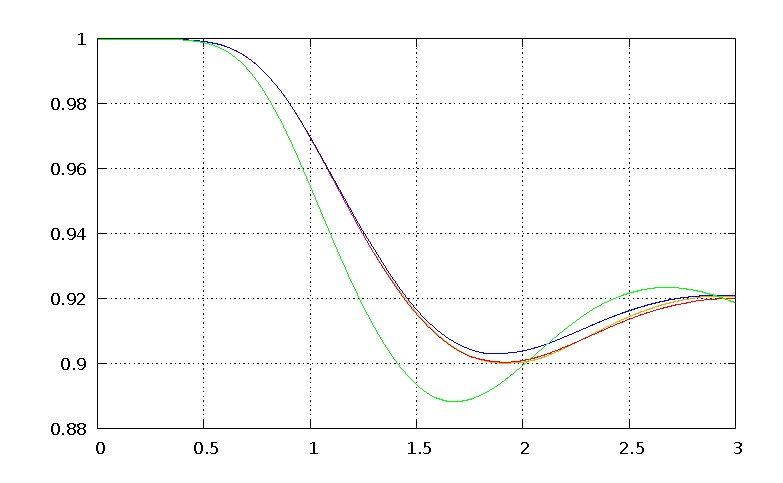
\includegraphics[width=.45\textwidth]
{figures/rising_bubble_I_sphericity.ps}
\caption[Navier--Stokes rising bubble I sphericity]
{A plot of the sphericity $\strikes$ over time for the simulation in
Figure~\ref{fig:risingbubbleIpressure} for the explicit (orange), implicit
(red), ALE (blue) and antisymmetric (green) schemes.}
\label{fig:risingbubbleIsphericity}
\end{figure}

\begin{figure}[htbp]
\centering
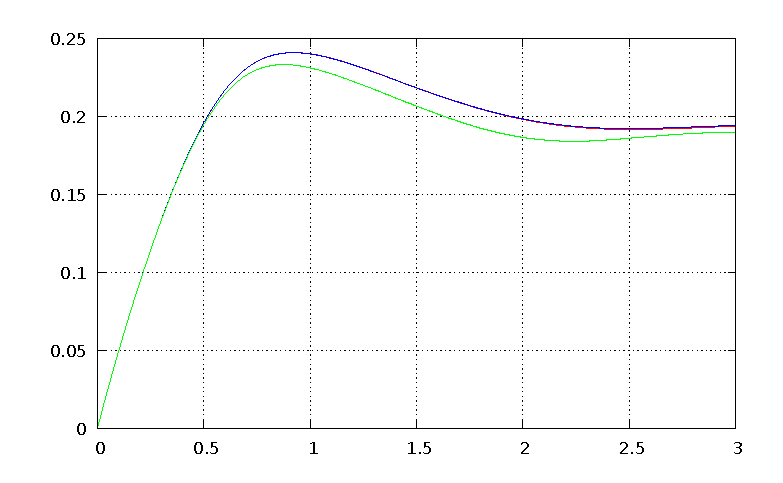
\includegraphics[width=.45\textwidth]
{figures/rising_bubble_I_rising_velocity.ps}
\caption[Navier--Stokes rising bubble I rising velocity]
{A plot of the rising velocity $V_c$ over time for the simulation in
Figure~\ref{fig:risingbubbleIpressure} for the explicit (orange), implicit
(red), ALE (blue) and antisymmetric (green) schemes.}
\label{fig:risingbubbleIrisingvelocity}
\end{figure}

\begin{figure}[htbp]
\centering
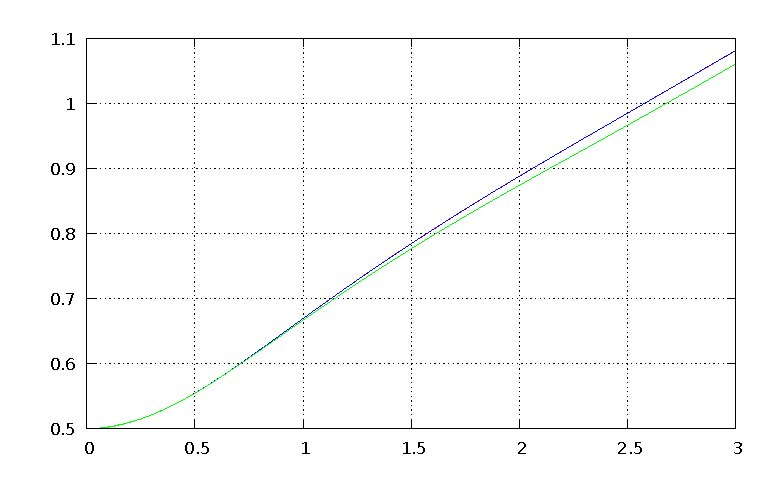
\includegraphics[width=.45\textwidth]
{figures/rising_bubble_I_barycenter.ps}
\caption[Navier--Stokes rising bubble I barycenter]
{A plot of the barycenter $z_c$ over time for the simulation in
Figure~\ref{fig:risingbubbleIpressure} for the explicit (orange), implicit
(red), ALE (blue) and antisymmetric (green) schemes.}
\label{fig:risingbubbleIbarycenter}
\end{figure}

\begin{figure}[htbp]
\centering
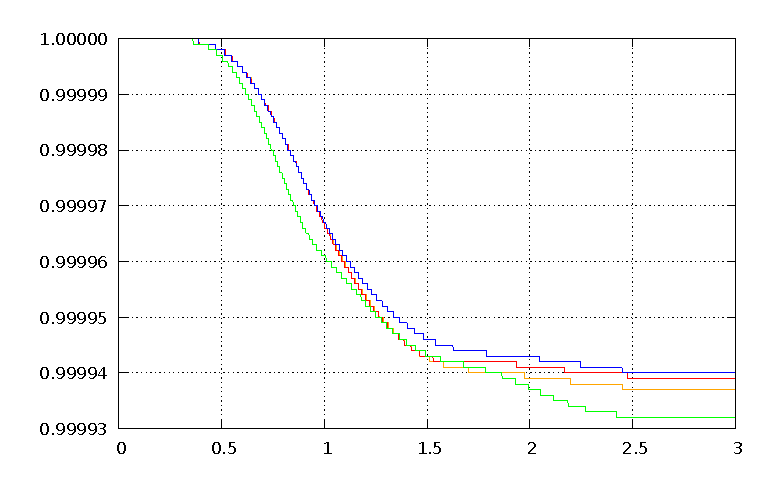
\includegraphics[width=.45\textwidth]
{figures/rising_bubble_I_inner_volume.ps}
\caption[Navier--Stokes rising bubble I inner area]
{A plot of the relative inner area
$\frac{\mathcal{L}^2(\Omega^m_-)}{\mathcal{L}^2(\Omega^0_-)}$ over time for the
simulation in Figure~\ref{fig:risingbubbleIpressure} for the explicit
(orange), implicit (red), ALE (blue) and antisymmetric (green) schemes.}
\label{fig:risingbubbleIinnervolume}
\end{figure}

The physical parameters for the rising bubble experiment II are
\begin{equation} \label{eq:Hysing2}
\rho_+ = 1000\,,\quad \rho_- = 1\,,\quad \mu_+ = 10\,,\quad \mu_- = 0.1\,,\quad
\gamma = 1.96\,,
\end{equation}
see the test case 2 in \cite[Table~I]{HysingTKPBGT09}. We report on
quantitative results for the rising bubble experiment II for the P2--\pdg and
P2--(P1+P0) elements in Table~\ref{tab:risingbubbleII}. See
\S\ref{sec:benchmark_quantities} for the definitions of the various benchmark
quantities. For each element, we compare the explicit, implicit and ALE scheme
derived in Chapter \ref{ch:navier_stokes} and Chapter \ref{ch:ale}. We use
$J_\Gamma=128$ interface elements with $J_\Omega^0=35092$ initial bulk elements.
The final number of bulk elements, $J_\Omega^M$, for the explicit scheme for
the P2--(P1+P0) element is 10638.
\begin{table*}
\center
\hspace*{-3.25cm}
\begin{tabular}{rll}
\hline
 & P2--\pdg & P2--(P1+P0) \\
\hline
& \multicolumn{2}{c}{explicit} \\
\cmidrule{2-3}
$\strikes_{\min}$                & 0.5412 & 0.5435 \\
$t_{\strikes = \strikes_{\min}}$ & 3.0000 & 3.0000 \\
$V_{c,\max 1}$                   & 0.2501 & 0.2503 \\
$t_{V_c = V_{c,\max 1}}$         & 0.7290 & 0.7290 \\
$V_{c,\max 2}$                   & 0.2402 & 0.2403 \\
$t_{V_c = V_{c,\max 2}}$         & 2.1030 & 2.1070 \\
$z_c(t=3)$                       & 1.1384 & 1.1383 \\
CPU                              & 128299 & 132498 \\
\cmidrule{2-3}
& \multicolumn{2}{c}{implicit} \\
\cmidrule{2-3}
$\strikes_{\min}$                & 0.5443 & 0.5473 \\
$t_{\strikes = \strikes_{\min}}$ & 3.0000 & 3.0000 \\
$V_{c,\max 1}$                   & 0.2501 & 0.2502 \\
$t_{V_c = V_{c,\max 1}}$         & 0.7290 & 0.7290 \\
$V_{c,\max 2}$                   & 0.2402 & 0.2403 \\
$t_{V_c = V_{c,\max 2}}$         & 2.1040 & 2.1540 \\
$z_c(t=3)$                       & 1.1385 & 1.1387 \\
CPU                              & 216605 & 236635 \\
\cmidrule{2-3}
& \multicolumn{2}{c}{ALE} \\
\cmidrule{2-3}
$\strikes_{\min}$                & - & 0.5266 \\
$t_{\strikes = \strikes_{\min}}$ & - & 3.0000 \\
$V_{c,\max 1}$                   & - & 0.2502 \\
$t_{V_c = V_{c,\max 1}}$         & - & 0.7300 \\
$V_{c,\max 2}$                   & - & 0.2400 \\
$t_{V_c = V_{c,\max 2}}$         & - & 2.0670 \\
$z_c(t=3)$                       & - & 1.1385 \\
CPU                              & - & 236253 \\
\hline
\end{tabular}
\hspace*{-3.25cm}
\caption[Navier--Stokes rising bubble II benchmark values]
{($\rho_+ = 1000,\rho_- = 1,\mu_+ = 10,\mu_- =0.1,\gamma = 1.96$)
Rising bubble experiment II on ${\Omega = (0,1) \times (0,2)}$ over the time
interval $[0,3]$, with nearly uniform meshes, $J_\Gamma=128$ and
$C_a=20\degree$.}
\label{tab:risingbubbleII}
\end{table*}
We observe that the results in Table~\ref{tab:risingbubbleII}
are in good agreement with the corresponding numbers from the finest
discretization run of group 3 in \cite{HysingTKPBGT09}, which are given by
0.5144, 3.0000, 0.2502, 0.7317, 0.2393, 2.0600 and 1.1376. Here we note that
there is little agreement on these results between the three groups in
\cite{HysingTKPBGT09}, but we believe the numbers of group 3 to be the most
reliable ones. Similar results are also obtained in \cite{fluidfbp}. Some
results in Table~\ref{tab:risingbubbleII} are missing because one simulation
had an early termination triggered by a bulk mesh overlap in the last steps.

In Figure~\ref{fig:risingbubbleIIpressure} we show the evolution of the discrete
pressures for a simulation with $J_\Gamma=128$ interface elements using the
P2--(P1+P0) element and the explicit scheme, while the velocities are visualized
in Figure~\ref{fig:risingbubbleIIvelocity}.
\begin{figure}[htbp]
\centering
\subfloat[$t=10^{-5}$]{\includegraphics[width=.45\textwidth]
{figures/rising_bubble_II_pressure_0.ps}}
\subfloat[$t=1$]{\includegraphics[width=.45\textwidth]
{figures/rising_bubble_II_pressure_1.ps}}\\
\subfloat[$t=2$]{\includegraphics[width=.45\textwidth]
{figures/rising_bubble_II_pressure_2.ps}}
\subfloat[$t=3$]{\includegraphics[width=.45\textwidth]
{figures/rising_bubble_II_pressure_3.ps}}
\caption[Navier--Stokes rising bubble II pressure]
{($\rho_+ = 1000,\rho_- = 1,\mu_+ = 10,\mu_- =0.1,\gamma = 1.96$)
Pressure evolution for the rising bubble experiment II for the P2--(P1+P0)
element and the explicit scheme, with nearly uniform mesh and
$C_a=20\degree$.}
\label{fig:risingbubbleIIpressure}
\end{figure}

\begin{figure}[htbp]
\centering
\subfloat[$t=10^{-5}$]{\includegraphics[width=.45\textwidth]
{figures/rising_bubble_II_velocity_0.ps}}
\subfloat[$t=1$]{\includegraphics[width=.45\textwidth]
{figures/rising_bubble_II_velocity_1.ps}}\\
\subfloat[$t=2$]{\includegraphics[width=.45\textwidth]
{figures/rising_bubble_II_velocity_2.ps}}
\subfloat[$t=3$]{\includegraphics[width=.45\textwidth]
{figures/rising_bubble_II_velocity_3.ps}}
\caption[Navier--Stokes rising bubble II velocity]
{($\rho_+ = 1000,\rho_- = 1,\mu_+ = 10,\mu_- =0.1,\gamma = 1.96$)
Velocity vector field for the rising bubble experiment II for the P2--(P1+P0)
element and the explicit scheme, with nearly uniform mesh and
$C_a=20\degree$.}
\label{fig:risingbubbleIIvelocity}
\end{figure}

In Figures~\ref{fig:risingbubbleIIsphericity},
\ref{fig:risingbubbleIIrisingvelocity} , \ref{fig:risingbubbleIIbarycenter} and
\ref{fig:risingbubbleIIinnervolume} are reported, respectively, the evolution of
the sphericity $\strikes$, rising velocity $V_c$, barycenter $z_c$ and relative
inner area $\frac{\mathcal{L}^2(\Omega^m_-)}{\mathcal{L}^2(\Omega^0_-)}$ over
time. We have used the P2--(P1+P0) element and $J_\Gamma=128$ interface
elements. In Figure~\ref{fig:risingbubbleIIinnervolume} we observe oscillations
in the relative inner area between $t=2.1$ and $t=2.3$. In that interval the
bubble assumes a more non-convex shape and develops thin filaments which
originate these oscillations.
\begin{figure}[htbp]
\centering
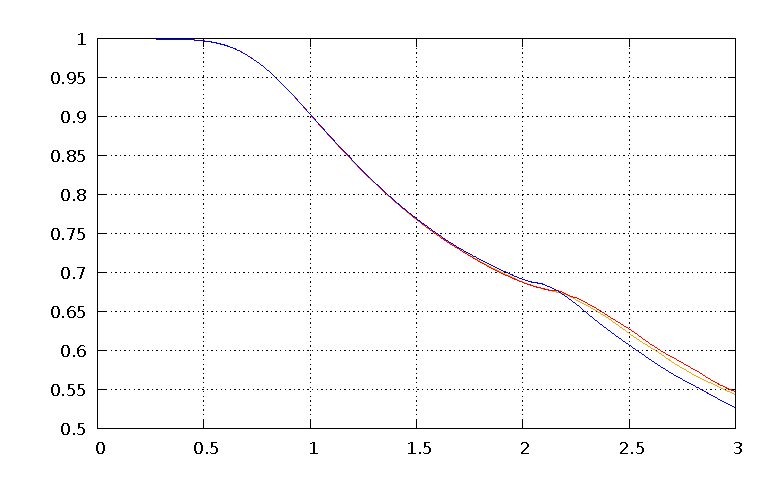
\includegraphics[width=.45\textwidth]
{figures/rising_bubble_II_sphericity.ps}
\caption[Navier--Stokes rising bubble II sphericity]
{A plot of the sphericity $\strikes$ over time for the simulation in
Figure~\ref{fig:risingbubbleIIpressure} for the explicit (orange), implicit
(red) and ALE (blue) schemes.}
\label{fig:risingbubbleIIsphericity}
\end{figure}

\begin{figure}[htbp]
\centering
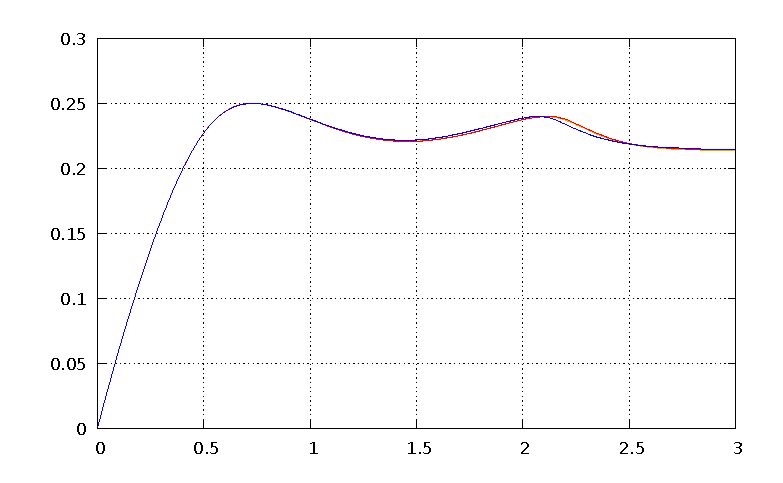
\includegraphics[width=.45\textwidth]
{figures/rising_bubble_II_rising_velocity.ps}
\caption[Navier--Stokes rising bubble II rising velocity]
{A plot of the rising velocity $V_c$ over time for the simulation in
Figure~\ref{fig:risingbubbleIIpressure} for the explicit (orange), implicit
(red) and ALE (blue) schemes.}
\label{fig:risingbubbleIIrisingvelocity}
\end{figure}

\begin{figure}[htbp]
\centering
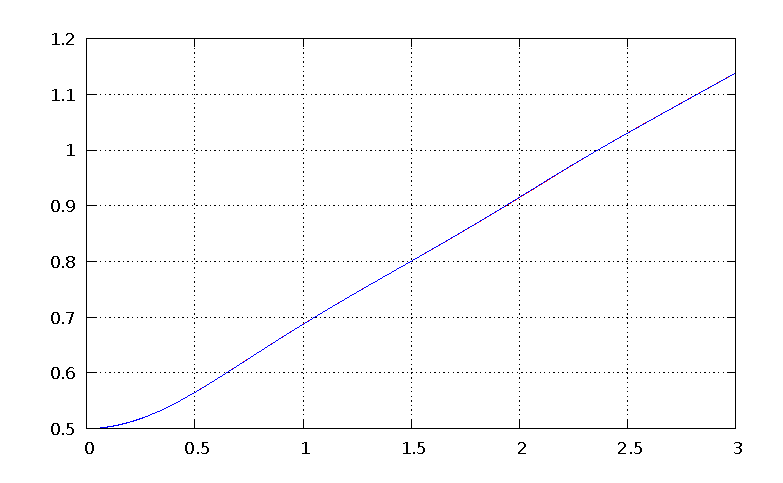
\includegraphics[width=.45\textwidth]
{figures/rising_bubble_II_barycenter.ps}
\caption[Navier--Stokes rising bubble II barycenter]
{A plot of the barycenter $z_c$ over time for the simulation in
Figure~\ref{fig:risingbubbleIIpressure} for the explicit (orange), implicit
(red) and ALE (blue) schemes.}
\label{fig:risingbubbleIIbarycenter}
\end{figure}

\begin{figure}[htbp]
\centering
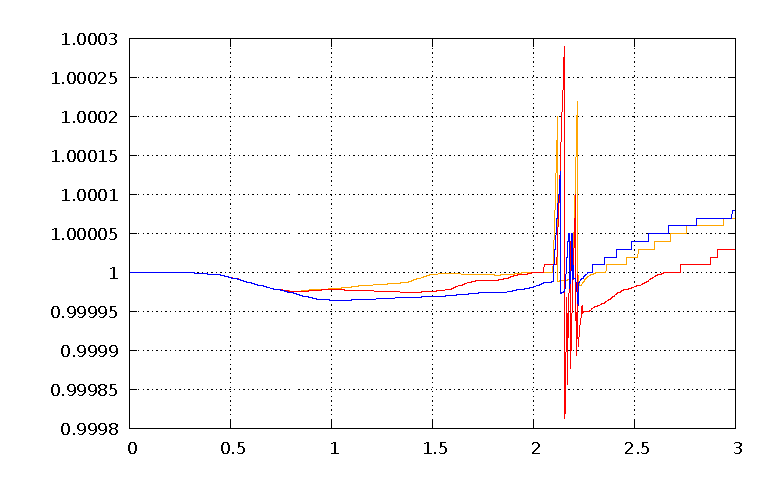
\includegraphics[width=.45\textwidth]
{figures/rising_bubble_II_inner_volume.ps}
\caption[Navier--Stokes rising bubble II inner area]
{A plot of the relative inner area
$\frac{\mathcal{L}^2(\Omega^m_-)}{\mathcal{L}^2(\Omega^0_-)}$ over time for the
simulation in Figure~\ref{fig:risingbubbleIIpressure} for the explicit
(orange), implicit (red) and ALE (blue) schemes.}
\label{fig:risingbubbleIIinnervolume}
\end{figure}

We finally notice that in both experiments, namely the rising bubble I and II,
the ALE scheme and the non-ALE schemes are all performing well. Therefore, the
downside of having to project the velocity in the non-ALE formulations seems to
be less severe than expected. This can be partly explained by the good
interface mesh, which never changes even after a full bulk remeshing.

\bibliographystyle{siam}
\bibliography{../../bib/robert_refs,../../bib/marco_refs}
\end{document}
